\documentclass{book}

\usepackage{ctex}
\usepackage{lipsum}
\usepackage{amsmath, amsthm, amssymb, amsfonts,mathrsfs}
\usepackage{thmtools}
\usepackage{graphicx}
\usepackage{setspace}
\usepackage{geometry}
\geometry{
  a4paper,
  top=25.4mm, bottom=25.4mm,
  left=20mm, right=20mm,
  headheight=2.17cm,
  headsep=4mm,
  footskip=12mm
}
\usepackage{float}
\usepackage{hyperref}
\usepackage[utf8]{inputenc}
\usepackage[english]{babel}
\usepackage{framed}
\usepackage[dvipsnames]{xcolor}
\usepackage{tikz-cd}
\usepackage[most]{tcolorbox}
\usepackage[UTF8]{ctex}
\usepackage{colortbl}
\usepackage{pifont}
\usepackage{framed}
\definecolor{shadecolor}{RGB}{241, 241, 255}
\newcounter{problemname}

\tcbuselibrary{theorems}
\tcbuselibrary{breakable}
\hypersetup{hidelinks,
	colorlinks=true,
	allcolors=black,
	pdfstartview=Fit,
	breaklinks=true
}

%定义颜色,可以根据需求自己修改
\definecolor{LightIndigo}{HTML}{E0FFFF}
\colorlet{LightGray}{White!90!Periwinkle}
\colorlet{LightOrange}{Orange!15}
\colorlet{LightGreen}{Green!15}
\colorlet{Lightblue}{Blue!15}
\colorlet{Lightpurple}{Purple!15}
\colorlet{LightRed}{Red!15}
\colorlet{LightYellow}{Yellow!15}
\colorlet{LightCyan}{Cyan!15}
%\colorlet{LightIndigo}{E0FFFF}

\newcommand{\HRule}[1]{\rule{\linewidth}{#1}}

\newtheorem{corollary}{Corollary}[section]
\newenvironment{solution}{{\noindent\it Solution.} }{\hfill $\square$\par}
\newenvironment{note}{\noindent\it Note.}{\par}

\declaretheoremstyle[name=Theorem,]{thmsty}
\declaretheorem[style=thmsty,numberwithin=section]{theorem}
\tcolorboxenvironment{theorem}{colback=LightGray,breakable,before upper app={\setlength{\parindent}{2em}}}

\declaretheoremstyle[name=Definition,]{thmsty}
\declaretheorem[style=thmsty,numberwithin=section]{definition}
\tcolorboxenvironment{definition}{colback=LightCyan,breakable,before upper app={\setlength{\parindent}{2em}}}

\declaretheoremstyle[name=Remark,]{thmsty}
\declaretheorem[style=thmsty,numberwithin=section]{remark}
\tcolorboxenvironment{remark}{colback=LightRed,breakable,before upper app={\setlength{\parindent}{2em}}}

\declaretheoremstyle[name=Lemma,]{thmsty}
\declaretheorem[style=thmsty,numberwithin=section]{lemma}
\tcolorboxenvironment{lemma}{colback=Lightblue,breakable,before upper app={\setlength{\parindent}{2em}}}

\declaretheoremstyle[name=Corollary,]{thmsty}
\declaretheorem[style=thmsty,numberwithin=section]{Corollary}
\tcolorboxenvironment{corollary}{colback=Lightpurple,breakable,before upper app={\setlength{\parindent}{2em}}}

\declaretheoremstyle[name=Proposition,]{prosty}
\declaretheorem[style=prosty,numberwithin=section]{proposition}
\tcolorboxenvironment{proposition}{colback=LightOrange,breakable,before upper app={\setlength{\parindent}{2em}}}

\declaretheoremstyle[name=Example,]{prosty}
\declaretheorem[style=prosty,numberwithin=section]{example}
\tcolorboxenvironment{example}{colback=LightGreen,breakable,before upper app={\setlength{\parindent}{2em}}}

\declaretheoremstyle[name=Exercise,]{prosty}
\declaretheorem[style=prosty,numberwithin=section]{exercise}
\tcolorboxenvironment{exercise}{colback=LightYellow,breakable,before upper app={\setlength{\parindent}{2em}}}

\setstretch{1.2}
\geometry{
    textheight=9in,
    textwidth=5.5in,
    top=1in,
    headheight=12pt,
    headsep=25pt,
    footskip=30pt
}
\usepackage{float}
\usepackage{enumitem}
\usepackage{amsmath}
\usepackage{amssymb}
\usepackage{hyperref}
\usepackage{cleveref}
\usepackage{annotate-equations}
\usepackage{zhlipsum}

\newcommand\tbbint{{-\mkern -16mu\int}}
\newcommand\tbint{{\mathchar '26\mkern -14mu\int}}
\newcommand\dbbint{{-\mkern -19mu\int}}
\newcommand\dbint{{\mathchar '26\mkern -18mu\int}}
\newcommand\bint{
{\mathchoice{\dbint}{\tbint}{\tbint}{\tbint}}
}
\newcommand\bbint{
{\mathchoice{\dbbint}{\tbbint}{\tbbint}{\tbbint}}
}


\linespread{1.5}
\title{ \normalsize \textsc{Notes of Fourier Research}
		\\ [2.0cm]
		\HRule{1.5pt} \\
		\LARGE \textbf{\uppercase{调和分析笔记}
		\HRule{2.0pt} \\ [0.6cm] \LARGE{Jinhua Wu} \vspace*{10\baselineskip}}
		}
\date{}
\author{}

\begin{document}
\maketitle
\tableofcontents 
\newpage
\setcounter{page}{1}
\chapter{Fourier级数和Fourier积分}
\paragraph{什么是调和分析?}
\begin{align*}
    \Delta u = 0 \quad \text{调和方程}
\end{align*}
方法:Fourier变换、Fourier级数。

\section{Fourier级数}
\begin{align*}
    f(x) &= \sum\limits_{k=0}^{\infty} a_k \cos (2\pi kx) + b_k \sin (2\pi kx) \\
    e^{iy} &= \cos y + i\sin y \\
    \eqnmarkbox[red]{1}{f(x)} &= \sum\limits_{k=-\infty}^{\infty} c_k e^{i2\pi kx}
\end{align*}
\annotate[yshift=0.5em]{above,left}{1}{什么时候可以满足?}

这里需要注意的是,我们可以对$\cos$与$\sin$进行变换,以$\{e^{ikx}\mid k\in\mathbb{Z}\}$为Basis,即
\begin{align*}
    \cos 2\pi k x &= \frac{e^{2\pi k x} + e^{-2\pi k x}}{2} \\
    \sin 2\pi k x &= \frac{e^{2\pi k x} - e^{-2\pi k x}}{2i} \\
\end{align*}


对$f$的要求:$f$在$\mathbb{R}$上以$1$为周期。若右边级数一致收敛,则
\begin{align*}
    \int_0^1 f(x) e^{-2\pi jx} &= \sum\limits_{k=-\infty}^{\infty} c_k \eqnmarkbox[red]{2}{\int_0^1 e^{i2\pi(k-j)x}dx} \\
    \text{where}\ \int_0^1 f(x)e^{-i2\pi jx}dx &= c_j
\end{align*}
\annotate[yshift=0.5em]{above,right}{2}{用了$\int_0^1 e^{2\pi i(k-j)x}dx = \left\lbrace\begin{array}{ll}
    0 & k\neq j \\
    1 & k = j
\end{array}\right.$}

记
\begin{align*}
    c_j &= \hat{f}(j) \\
    \text{where}\ \hat{f}(j) &\triangleq \int_0^1 f(x) e^{-2\pi jx}dx 
\end{align*}

\vspace{1em}
$\eqnmark[red]{3}{f\in L^1([0,1])}$,$f$定义在$\mathbb{R}$上,以$1$为周期,且$f:\mathbb{R}\to\mathbb{R}$。这里简记为$\eqnmarkbox[red]{10}{f\in L^1(\mathbb{T})}$\footnote{$f\in C(\mathbb{T})$,指$f\in\mathbb{R}$,周期为$1$,$f$在$\mathbb{R}$上连续},其中$\mathbb{T} = \mathbb{R}/\mathbb{Z}$。
\annotate[yshift=0.5em]{above,right}{3}{这里研究的都是Lesbegue可积,不同于数学分析中的Riemann}
\annotate[yshift=-0.5em]{below,left}{10}{$f:\mathbb{R}\to\mathbb{R}$,且$f$的周期为$1$,$f\in L^1[0,1)$。若换成$L^p$亦如此。}

这里$\mathbb{T}$可以被看作是实数$\mathbb{R}$模$1$的商集。 在这个定义下,\(\mathbb{T}\) 的元素可以通过对实数取模运算(即 \( x \mod 1 \))来表示,因此它形成了一个加法群,即在单位圆上通过加法操作可以得到新的元素。

\(\mathbb{T}\) 被称为一维环面(one-dimensional torus),表示它是一种拓扑空间,可以被看作是单位圆的几何表示。即:
  \[
  \mathbb{T} = \{ z \in \mathbb{C} \mid |z| = 1 \}
  \]
  或者可以表示为:
  \[
  \mathbb{T} = \{ e^{2\pi i x} \mid x \in [0,1) \}
  \]
  这意味着我们可以通过在复平面上绘制单位圆来理解 \(\mathbb{T}\),其中每个点的相位角与区间 \([0,1)\) 中的实数 \(x\) 一一对应。这个拓扑解释帮助我们理解\(\mathbb{T}\) 的连续性和周期性。作为环面,它不仅有群结构,还可以定义各种拓扑和几何性质,例如我们可以在 \(\mathbb{T}\) 上定义距离、度量等。

\section{Fourier级数的点态收敛}
$n$项对称和:
\begin{align*}
    S_Nf(x) \triangleq \sum\limits_{k=-N}^{N} \hat{f}(k) e^{2\pi ikx}
\end{align*}
当然,我们也可以以最初的形式来书写,即
\begin{align*}
    S_N f(x) = \sum\limits_{k=-N}^{N} a_k \cos (2\pi kx) + b_k \sin (2\pi kx)
\end{align*}

问:当$f$满足什么条件的时候,$S_N f(x)$的极限存在?
\begin{align*}
    S_N f(x) &= \sum\limits_{k=-N}^N \int_0^1 f(t) e^{-2\pi ikt} dt \cdot e^{2\pi ikx} \\
    & = \int_0^1 f(t) \eqnmarkbox[red]{4}{\sum\limits_{k=-N}^N e^{2\pi ik(x-t)}} dt \\
    & = \int_0^1 \eqnmarkbox[red]{5}{f(t) D_N(x-t)} dt = \int_0^1 f*D_N dt \\
    \text{where}\ D_N(t) &= \sum\limits_{k=-N}^N e^{2\pi ikt}
\end{align*}
\annotate[yshift=0.5em]{above,right}{4}{$D_N(x-t)$,称为Dirichlet核}
\annotate[yshift=-0.5em]{below,right}{5}{周期为$1$}

这里我们可以看出求和与积分交换是基于Lebesgue逐项积分定理,见实变函数P43:
\begin{theorem}
    \color{blue}
    设$\{f_k\}$是$E\subset \mathbb{R}^n$上的非负可测函数列,记
    \begin{align*}
        f(x)\triangleq \sum\limits_{k=0}^{\infty} f_k(x) \quad (x\in E)
    \end{align*}
    则$\sum\limits_{k=0}^{\infty} f_k(x)$可逐项积分,即
    \begin{align*}
        \int_E f(x) dx \triangleq \int_E \sum\limits_{k=0}^{\infty} f_k(x) dx \triangleq \sum\limits_{k=0}^{\infty} \int_E f_k(x) dx
    \end{align*}
\end{theorem}
\begin{proof}
    \color{blue} 这里的证明是自然的,我们令
    \begin{align*}
        S_n(x) \triangleq \sum\limits_{k=0}^{n} f_k(x)
    \end{align*}
    即$\{S_n(x)\}$为单调递增列,因而由Levi即得。
\end{proof}

其中
\begin{align*}
    D_N(t) &= \frac{e^{-2\pi iNt}\left(1 - \left(e^{2\pi it}\right)^{2N+1} \right)}{1-e^{2\pi it}} \\
    &= \frac{e^{-2\pi iNt}(1-e^{2\pi i t (2N+1)})}{1 - e^{2\pi it}} \\
    & = \frac{e^{-2\pi iNt} - e^{2\pi i t(N+1)}}{1 - e^{2\pi i t}} \cdot \frac{e^{-\pi i t}}{e^{-\pi i t}} \\
    & = \frac{e^{-2\pi i t\left(N+\frac{1}{2}\right)} - e^{2\pi i t \left(N + \frac{1}{2}\right)}}{e^{-\pi i t} - e^{\pi i t}} \\
    & = \frac{2i \sin\left(2\pi t \left(N+ \frac{1}{2}\right)\right)}{ -2i \sin \pi t} \\
    & = \frac{\sin (2\pi t(N+\frac{1}{2})}{\sin \pi t}
\end{align*}

而考虑$t=0$之后得到
\begin{align*}
    D_N(t) &\triangleq \left\lbrace\begin{array}{ll}
        \frac{\sin (2\pi t(N + \frac{1}{2}))}{\sin \pi t} & t\neq 0 \\
        2N + 1 & t = 0
    \end{array} \right.
\end{align*}

\paragraph{$D_N(t)$的性质}
\begin{enumerate}[leftmargin=1cm, label=\arabic*]
    \item $D_N(t+1) = D_N(t)$;
    \item $\int_0^1 D_N(t) dt = 1$;
    \item $|D_N(t)| \leqslant \frac{1}{\sin\pi\delta}$,$\delta\leqslant |t| \leqslant \frac{1}{2}$,$\delta>0$;
    \item $D_N(-t) = D_N(t)$
\end{enumerate}

由于$f\in L^1(\mathbb{T})$,所以这里我们仅需取周期为1的一个区间即可。
\begin{align*}
    D_Nf(t) &= \int\limits_{-\frac{1}{2}}^{\frac{1}{2}} f(t) D_N(x-t) dt \\
    &= \int\limits_{-\frac{1}{2}}^{\frac{1}{2}} D_N(t) f(x-t) dt
\end{align*}

\begin{theorem}[Dini判别法]
    $f\in L^1(\mathbb{T})$,$x\in[0,1]$,若$\exists \delta>0$,满足
    \begin{align*}
        \int\limits_{|t|<\delta} \frac{|f(x+t) - f(x)|}{|t|} dt < \infty
    \end{align*}
    则$S_N f(x) \to f(x)$,当$N\to+\infty$。
\end{theorem}

\begin{proof}
    \begin{align*}
        S_N f(x) - f(x) &= \int\limits_{-\frac{1}{2}}^{\frac{1}{2}} f(x-t) D_N(t) dt - f(x)\int\limits_{-\frac{1}{2}}^{\frac{1}{2}} D_N(t) dt \\
        & = \int\limits_{|t|<\delta} \left(\frac{f(x-t) - f(x)}{t} \frac{t}{\sin(\pi t)}\right) \eqnmark[red]{1}{\sin\pi(t)(2N + 1)} dt + \int\limits_{\delta\leqslant |t| \leqslant \frac{1}{2}} [f(x-t) - f(x)] \frac{\sin(\pi t(2N+1))}{\sin(\pi t)}dt \\
        & \to 0
    \end{align*}
    \annotate[yshift=0.5em]{below,right}{1}{$\to 0$}
\end{proof}

\begin{remark} 
    \begin{enumerate}
        \item 更进一步的,若满足Hölder条件,即
    \begin{align}
        |f(x+t) - f(x)| < t^{\alpha},\quad \alpha>0 \label{eq-1}
    \end{align}
    则显然满足Dini条件。若将(\ref{eq-1})的右侧改为$\frac{1}{(\ln t)^p}$,其中$p>1$,亦满足Dini条件。
    \item $f$在$x$连续,不能推出Dini条件。
    \end{enumerate}
\end{remark}



\begin{theorem}[Dirichlet-Jordan判别法]
    $f\in L(\mathbb{T})$,若$\exists \delta > 0$,s.t.
    \begin{align*}
        f\in \text{BV}([x-\delta,\ x+\delta]) \quad \text{有界变差函数}
    \end{align*}
    则$S_N f(x) \to \frac{f(x+0) + f(x-0)}{2}$,当$N\to\infty$。
\end{theorem}
\begin{proof}
    \begin{enumerate}[leftmargin=1cm, label=\arabic*]
        \item 先设$f$在$[x_0-\delta,x_0+\delta]$上单调,则
        \begin{align*}
            S_N f(x_0) &= \int\limits_{-\frac{1}{2}}^{\frac{1}{2}} f(x_0 - t) D_N(t) dt \\
            & = \int\limits_{0}^{\frac{1}{2}} f(x_0-t) D_N(t) dt + \int\limits_{-\frac{1}{2}}^0 f(\eqnmark[red]{1}{x_0-t}) D_N(t) dt \\
            & = \int\limits_0^{\frac{1}{2}} \left(f(x_0-t) + f(x_0 + t) \right) D_N(t) dt
        \end{align*}
        \annotate[yshift=0.5em]{above,right}{1}{$=s$}

        \noindent\textbf{断言}:若$g(t)$在$[0,\delta]$单调,则
        \begin{align*}
            \lim\limits_{N\to\infty} \int\limits_{0}^{\frac{1}{2}} g(t) D_N(t) dt = \frac{1}{2} g(0+)
        \end{align*}
        \begin{proof}
            先设$g$在$[0,\delta]$上单调递增,则
            \begin{align*}
                \int\limits_0^{\frac{1}{2}} g(t)D_N(t) dt - \frac{1}{2}g(0+) &= \int\limits_0^{\frac{1}{2}} g(t) D_N(t) - \int\limits_0^{\frac{1}{2}} g(0+) D_N(t) dt \\
                & = \int\limits_0^{\frac{1}{2}} (g(t) - g(0+)) D_N(t) dt \\
                & = \int\limits_0^{\delta} (g(t) - g(0+)) D_N(t) dt + \int\limits_{\delta}^{\frac{1}{2}} \left[\frac{(g(t) - g(0+))}{\sin \pi t}\chi_{[\delta,\frac{1}{2}]}(t)\right]  \sin \pi t(2N+1) dt \\
                & = \int\limits_0^{\delta} \eqnmark[red]{a1}{(g(t) - g(0+))} \eqnmark[blue]{a2}{\frac{\sin\pi t(2N+1)}{\sin\pi t}} dt \\
                & + \int\limits_{\delta}^{\frac{1}{2}} \eqnmark[green]{a3}{\left[\frac{(g(t) - g(0+))}{\sin \pi t}\chi_{[\delta,\frac{1}{2}]}(t)\right]}  \sin \pi t(2N+1) dt \\
                & \triangleq I + II
            \end{align*}
            \annotate[yshift=0.5em]{above,right}{a1}{$\geqslant 0$}
            \annotate[yshift=0.5em]{below,right}{a2}{$\in C[0,\delta]$}
            \annotate[yshift=0.5em]{above,right}{a3}{$\to 0$}
            
            \begin{align*}
                I \underset{\text{积分第二中值定理}}{\Longrightarrow}\ \eqnmark[red]{b1}{\left(g(\delta) - g(0)\right)} \eqnmark[blue]{b2}{\int\limits_{\xi}^{\delta} \frac{\sin\pi t(2N+1)}{\sin \pi t} dt}
            \end{align*}
            \annotate[yshift=0.5em]{above,right}{b1}{$< \varepsilon$}
            \annotate[yshift=0.5em]{above,right}{b2}{$\leqslant C$,不依赖于$N$}
            其中
            \begin{align*}
                \int\limits_{\xi}^{\delta} \frac{\sin\pi t(2N+1)}{\sin \pi t} dt & = \int_{\xi}^{\delta} \sin(\pi t(2N+1)) \left(\frac{1}{\sin(\pi t)} - \frac{1}{\pi t} \right) dt + \frac{1}{\pi} \int\limits_{\xi}^{\delta} \frac{\sin(\pi t(2N+1))}{\pi t(2N+1)} dt(2N+1) \\
                \frac{1}{\pi} \left|\int\limits_a^b \frac{\sin u}{u} du \right| &\leqslant \frac{6}{\pi} \\
                \left|\frac{1}{\pi t} - \frac{1}{\sin \pi t}\right| & = \frac{|\sin(\pi t) - \pi t|}{|(\pi t) - \sin(\pi t)|} \leqslant \frac{\frac{1}{2} (\pi t)^2}{(\pi t)\sin(\pi t)} \leqslant \frac{\pi}{4}
            \end{align*}

            而若$g(t)$单调下降,则考虑$-g(t)$是单调上升的,从而对单调函数均可满足。
        \end{proof}

        若断言成立,则
        \begin{align*}
            \lim\limits_{N\to\infty}\int\limits_0^{\frac{1}{2}} f(x_0-t) D_N(t) dt &= \frac{1}{2} f(x_0-) \\
            \lim\limits_{N\to\infty}\int\limits_0^{\frac{1}{2}} f(x_0+t) D_N(t) dt &= \frac{1}{2} f(x_0+)
        \end{align*}

        \item 由于$f\in\text{BV}[x_0-\delta,x_0+\delta]$,则
        \begin{align*}
            f &= f_1 - f_2 \\
            \text{where}\ & f_i\ \text{单调上升}
        \end{align*}
        从而
        \begin{align*}
            S_N(f)(x_0) &= S_N(f_1 - f_2)(x_0) = S_N(f_1)(x_0) - S_N(f_2)(x_0) \\
            & = \frac{1}{2}(f_1(x_0+0) + f_1(x_0-0)) - \frac{1}{2}(f_2(x_0+0) + f_2(x_0-0)) \\
            & = \frac{1}{2}(f(x_0+0) + f(x_0-0))
        \end{align*}
    \end{enumerate}
\end{proof}
\begin{remark}
    $f\in \text{BV}[a,b]$,当且仅当$f = f_1 - f_2$,其中$f_1$, $f_2$均为单调上升函数。
\end{remark}

\begin{remark}
    $f$是否收敛仅与$f$在这一点附近的邻域内的性质有关,见下述定理。
\end{remark}

\begin{theorem}[Riemann局部化]
    若$f\in L^1(\mathbb{T}$,$f(t)=0$,$t\in[x-\delta,x+\delta]$,则
    \begin{align*}
        S_N f(x) \to 0,\quad \text{when}\ N\to \infty
    \end{align*}
\end{theorem}
\begin{proof}
    \begin{align*}
        S_N f(x) &= \int\limits_{-\frac{1}{2}}^{\frac{1}{2}} f(x-t) D_N(t) dt \\
        &= \int\limits_{|t|>\delta} f(x-t) \frac{\sin(\pi t(2N+1))}{\sin(\pi t)} dt + \eqnmarkbox[red]{2}{\int\limits_{|t|\leqslant\delta} f(x-t) \frac{\sin(\pi t(2N+1))}{\sin(\pi t)} dt} \\
        & = \int\limits_{|t|>\delta} \frac{f(x-t)}{\sin(\pi t)} \left(\frac{e^{i\pi t(2N+1)} - e^{{2\pi t(2N+1)}}}{2i}\right) dt \\
        & = \frac{1}{2i} \int\limits_{|t|>\delta} \eqnmark[red]{3}{e^{i\pi t} \frac{f(x-t)}{\sin(\pi t)}} e^{i2\pi t} dt - \frac{1}{2i} \int\limits_{|t|>\delta} \eqnmark[red]{4}{e^{i\pi t} \frac{f(x-t)}{\sin(\pi t)}} e^{-i2\pi t} dt \\
        & \to 0 - 0 = 0
    \end{align*}
    \annotate[yshift=0.5em]{above,right}{2}{$=0$}
    \annotatetwo[yshift=-0.5em]{below,right}{3}{4}{$\leqslant\frac{|f(x-t)|}{\sin\pi\delta}$}
\end{proof}



\begin{theorem}[Riemann-Lesbegue引理]\label{tho-4}
   $f\in L^1(\mathbb{T})$,则
   \begin{align*}
       \lim\limits_{|k|\to\infty} \hat{f}(k) = 0
   \end{align*}

   可推广为
   \begin{align*}
       \lim\limits_{|\lambda|\to\infty} \hat{f}(\lambda) = 0
   \end{align*}
\end{theorem}
\begin{proof}
    当$f\in L^1([-1,2])$时,
    \begin{align}
        \hat{f}(k) &= \int\limits_0^1 f(t) e^{-2\pi ikt} dt \label{eq-2} \\
        &= -\int\limits_0^1 f(t) e^{-2\pi i kt} e^{-\pi i} dt \nonumber \\
        &= -\int\limits_0^1 f(t) e^{-2\pi ik\eqnmarkbox[red]{1}{\left(t + \frac{1}{2k}\right)}}dt \nonumber \\
        & = -\int\limits_{0}^1 f\left(s - \frac{1}{2k}\right) e^{-2\pi i ks}ds \label{eq-3}
    \end{align}
    \annotate[yshift=0.5em]{above,right}{1}{$=s$}

    因此
    \begin{align}
        |\hat{f}(k)| \leqslant \frac{1}{2} \cdot \int\limits_0^1 \left|  f(t) - f\left(t - \frac{1}{2k}\right) \right| \to 0,\quad \text{when}\ |k|\to + \infty \label{eq-4}
    \end{align}\footnote{这里是将(\ref{eq-2})与(\ref{eq-3})相加除以2即得(\ref{eq-4})}
\end{proof}


\subsection*{Homework 10th Sep}
\begin{example}
    证明,$\exists C > 0$
    \begin{align*}
        \sup\limits_{0\leqslant a< b} \left|\int\limits_a^b \frac{\sin t}{t} dt \right| \leqslant C
    \end{align*}
\end{example}
\begin{proof}
    分为两步,第一步说明$a=0$的情况成立,即
    \begin{align*}
        \int_0^b \frac{\sin t}{t} dt\to \int_0^{\infty} \frac{\sin t}{t}dt = \frac{\pi}{2},\quad \text{when}\ b \to \infty
    \end{align*}

    下面说明
    \begin{align*}
        \left|\int_a^b \frac{\sin t}{t}dt \right| \leqslant \left|\left|\int_0^b \frac{\sin t}{t}dt\right| - \left|\int_0^{\infty} \frac{\sin t}{t} dt \right|  \right| \leqslant 2M
    \end{align*}
    即可。
\end{proof}

\begin{example}
    举例说明Dini判别法,Jordan判别法的条件互不包含。
\end{example}
\begin{proof}
    前者利用$\sin\left(\frac{1}{x}\right)$,而后者利用跳跃分段函数即可。
\end{proof}


\section{连续函数的Fourier级数}
\begin{theorem}[Du Bios-Reymond]
    $\exists f\in C(\mathbb{T})$,s.t. $f$的Fourier级数在某一点发散。
\end{theorem}
\begin{proof}
    我们利用共鸣定理\footnote{\color{red} 共鸣定理:$\mathscr{X}$为Banach空间,$\mathscr{Y}$是$B^*$空间,$\forall \alpha\in\Gamma$,$T_{\alpha}\in\mathscr{L}(\mathscr{X},\mathscr{Y})$,若满足$\forall f\in\mathscr{X}$,$\sup\limits_{\alpha\in\Lambda} \|T_{\alpha} f\|<\infty$,则$\exists M>0$使得$\|T_{\alpha}f\| \leqslant M\|f\|$。},$\mathscr{X} = C(\mathbb{T})$,$\mathscr{Y} = \mathbb{C}$,$\|f\|_{C(T)} = \max\limits_{x\in[0,1]} |f(x)|$,定义算子
    \begin{align*}
        T_N f & \triangleq S_N f(0) = \int\limits_{-\frac{1}{2}}^{\frac{1}{2}} f(t) D_N(t) dt \\
        T_N &: \mathscr{X}\to\mathscr{Y}\ \text{线性} \\
        \|T_N f\| & = |S_N f(0)| \leqslant \int\limits_{-\frac{1}{2}}^{\frac{1}{2}} |f(t)| |D_N(t)| dt \leqslant \eqnmark[red]{c1}{\left(\int\limits_{-\frac{1}{2}}^{\frac{1}{2}} |D_N(t)| dt \right)} \|f\|_{\mathscr{X}} 
    \end{align*}
    \annotate[yshift=0.5em]{above,right}{c1}{$\frac{|\sin (\pi t(2N+1))|}{|\sin \pi t|} \leqslant\left\lbrace \begin{array}{ll}
        (2N+2) & B(0,\delta)  \\
        \frac{1}{\sin\pi\delta} & \text{远}
    \end{array}\right.$}
    从而$T_N\in\mathscr{L}(\mathscr{X},\mathscr{Y})$。断言:
    \begin{align*}
        \|T_N\| \overset{1}{=} \int\limits_{-\frac{1}{2}}^{\frac{1}{2}} |D_N(t)|dt \overset{2}{=} \frac{4}{\pi^2}\log N + O(1)
    \end{align*}
    若断言得证,则由共鸣定理,
    \begin{align*}
        \exists f_0\in C(\mathbb{T}) \quad s.t.\ \sup\limits_N \|T_N f_0\| = +\infty
    \end{align*}

    \paragraph{1} 
    \begin{align*}
        \|T_N\| = \int\limits_{-\frac{1}{2}}^{\frac{1}{2}} |D_N(t)|dt
    \end{align*}
    \begin{proof}
        \begin{align*}
            (i)\ \|T_N\| &\leqslant \int\limits_{-\frac{1}{2}}^{\frac{1}{2}} |D_N(t)|dt \\
            (ii)\ \forall \epsilon > 0,\ \|T_N\| & \geqslant \int\limits_{-\frac{1}{2}}^{\frac{1}{2}} |D_N(t)|dt - \varepsilon
        \end{align*}

        即找$\Tilde{f}$,s.t. $\Tilde{f}\in C(\mathbb{T})$,且
        \begin{align*}
            \|\Tilde{f}\|_{C(\mathbb{T})} = 1,\quad \text{and} \quad |T_N \Tilde{f}| \geqslant \int\limits_{-\frac{1}{2}}^{\frac{1}{2}} |D_N(t)|dt - \varepsilon
        \end{align*}

        而
        \begin{align*}
            T_N \Tilde{f} &= \int\limits_{-\frac{1}{2}}^{\frac{1}{2}} D_N(t) \Tilde{f}(t) dt \\
            &= \int\limits_{-\frac{1}{2}}^{\frac{1}{2}} D_N(t) \text{sgn}(D_N(t)) dt + \underbrace{\int\limits_{-\frac{1}{2}}^{\frac{1}{2}} D_N(t) \eqnmark[red]{d1}{(\Tilde{f}(t) - \text{sgn}(D_N(t)))} dt}\limits_{<\varepsilon}
        \end{align*}
         \annotate[yshift=0.5em]{above,right}{d1}{$\leqslant 2$}

        而由于
        \begin{align*}
            D_N(t) &= \frac{\sin(\pi t(2N+1)}{\sin \pi t}, \\
            |t| &\leqslant \frac{1}{2}
        \end{align*}

        而对于$\text{sgn}(D_N(t))$来说,不连续的点均在取值为$0$的地方,即
        \begin{align*}
            \pi t (2N+1) &= k\pi \\
            t & = \frac{k}{2N+1} \quad k = 1,2,\cdots
        \end{align*}
    \end{proof}

    \paragraph{2}
    \begin{proof}
        \begin{align*}
            \int\limits_{-\frac{1}{2}}^{\frac{1}{2}} |D_N(t)| dt & = 2\int\limits_0^{\frac{1}{2}} \frac{|\sin(\pi t(2N+1))|}{|\sin(\pi t)|} \frac{1}{2N+1} d(2N+1)t + \eqnmarkbox[red]{d3}{2\int\limits_{0}^{\frac{1}{2}} \left(\frac{1}{|\sin \pi t|} - \frac{1}{|\pi t|} \right) dt} \\
            & = 2\int\limits_{0}^{N+\frac{1}{2}} \frac{|\sin\pi u|}{\pi u} du + O(1) \\
            & = \frac{2}{\pi} \sum\limits_{k=0}^N \int\limits_{k}^{k+1} \frac{|\sin\pi u}{u} du + O(1) \\
            & = \frac{2}{\pi} \sum\limits_{k=1}^N \int\limits_0^1 \frac{|\sin\pi t|}{t+k} dt + O(1)\\ 
            & = \frac{2}{\pi} \int\limits_0^1 \sin(\pi t) \sum\limits_{k=1}^N \frac{1}{t+k} dt + O(1) \\
            & = \frac{2}{\pi } \int\limits_0^1 \sin(\pi t) \sum\limits_{k=1}^N (\ln N + O(1)) dt + O(1) \\
            & = \left(\frac{2}{\pi}\right)^2 \ln N + O(1)
         \end{align*}
        \annotate[yshift=0.5em]{above,left}{d3}{$O(1)$}
        
    \end{proof}
\end{proof}

\begin{remark}
    更进一步,$\exists\Tilde{f}\in C(\mathbb{T})$,s.t. $f$的Fourier级数在一个点列$\{x_k\}_{k=1}^{\infty}$上发散。
\end{remark}

% 19th Sep
\newpage
\section{Fourier级数按$L^p$收敛}
\begin{enumerate}[leftmargin=1cm, label=\arabic*]
    \item[Q1] $f\in L^p(\mathbb{T})\ (1\leqslant p< \infty)$,$\|S_N f - f\|_p \to \infty$,当$N\to\infty$;
    \item[Q2] $f\in L^p(\mathbb{T})$,$\lim\limits_{N\to\infty} S_N f(x) = f(x)$,a.e. $x\in\mathbb{T}$。
\end{enumerate}

考虑若$f\in C(\mathbb{T})$,那么是否有$S_N f(x)\to f(x)$,a.e. $x\in\mathbb{T}$? 1926,Kolmorgorov $\exists f\in L^1(\mathbb{T})$,$S_N f(x)$发散,$\forall x\in\mathbb{T}$。1965,Carleson,$f\in L^2(\mathbb{T})$,则$S_N f(x)\to f(x)$ a.e. $x\in\mathbb{T}$。1967,Hunt,$f\in L^p(\mathbb{T})$,$1<p<\infty$。

1917,Lusin猜想,$f\in L^2(\mathbb{T}^n)$,则$S_N f\to f$,a.e. $x\in\mathbb{T}^n$?

\begin{lemma}
    $1\leqslant p<\infty$,则$\|S_N f - f\|_p\to 0$,当且仅当$\exists C_p > 0$,s.t. $\|S_N f\|_p \leqslant C_p\|f\|_p$,这里$C_p$是不依赖于$N$与$f$的常数。
\end{lemma}                                                                \begin{proof}
    先证明$\Longrightarrow$,用共鸣定理(Banach-Steinhous),$\mathscr{X} = \mathscr{Y} = L^p(\mathbb{T})$,$S_N f = D_N * f$。且$S_N:\mathscr{X}\to\mathscr{Y}$为线性有界算子,则
    \begin{align*}
        \|S_N f\|_p &\leqslant L_N \|f\|_p \\
        \text{where}\ L_N &= \|D_N\|_p = \int\limits_{-1/2}^{1/2} |D_N(t)| dt = \frac{4}{\pi^2} \log N + O(1)
    \end{align*}
    从而$S_N f\overset{L^p}{\to} If$,$\forall f\in L^p$。

    再证明$\Longleftarrow$,
    \begin{enumerate}[leftmargin=1cm, label=\arabic*]
        \item 三角多项式:
        \begin{align*}
            \left\lbrace \sum\limits_{k=N_1}^{N_2} C_k e^{2\pi ikx}:\ N_1,N_2\in\mathbb{Z}\right\rbrace
        \end{align*}    

        三角多项式在$L^p\ (1\leqslant p<\infty)$中稠密,从而$\forall\varepsilon>0$,$\exists \varphi$在三角多项式中,$\|f-\varphi\|_p<\varepsilon$;

        \item $\forall\varphi\in$三角多项式,
        \begin{align*}
            \|\eqnmark[red]{a1}{S_N(\varphi)} - \varphi\|_p \to 0,\quad \text{when}\ N\to\infty
        \end{align*}
        \annotate[yshift=0.5em]{above,right}{a1}{$\to\varphi$}

        \item 由于$\|S_Nf\|_p \leqslant C_p\|f\|_p$,则
        \begin{align*}
            \|S_N f - f\|_p &\leqslant \|S_N f - S_N \varphi\|_p + \| S_N\varphi - \varphi\|_p + \|\varphi - f\|_p \to 0
        \end{align*}
    \end{enumerate}
\end{proof}

当$1< p<\infty$时(下述条件不满足$p=1$)
\begin{align*}
    S_N f = \frac{i}{2} \left(M_{-N}HM_{N} - M_N H M_{-N} \right)f
\end{align*}
其中$M_a f = e^{2\pi i x\cdot a} f(x)$,$H$为Hilbert变换,$\|H(f)\| \leqslant C_p\|f\|_p$,$1<p<\infty$(Chap 2-3),从而
\begin{align*}
    \|S_N f\|_p \leqslant \Tilde{C}_p \|H M_M f\|_p \leqslant \Tilde{C}_p C_p \|M_N f\| \leqslant \Tilde{C}_p C_p \|f\|_p
\end{align*}

$p=2$时,
\begin{align*}
    \|S_N f\|_2 &= \left|\sum\limits_{k=-N}^{N} \hat{f}(k) e^{2\pi i k x} \right|_2 \\
    &= \left(\sum\limits_{k=-N}^N |\hat{f}(k)|^2 \right)^{\frac{1}{2}} \\
    & \leqslant \left(\sum\limits_{k=-\infty}^{\infty} |\hat{f}(k)|^2 \right)^{\frac{1}{2}} \\
    & = \|f\|_{L^2}
\end{align*}


\newpage
\section{两种Fourier级数的求和法}
\begin{enumerate}[leftmargin=1cm, label=\arabic*]
    \item 算数平均求和($C_1$求和)
    \item Abel求和
\end{enumerate}

\subsection{算数求和}
\begin{definition}[算数平均求和]
    \begin{align*}
        \sigma_N f(x) &= \frac{1}{N+1} \sum\limits_{k=0}^N S_k f(x) \\
        &= \int\limits_{-\frac{1}{2}}^{\frac{1}{2}} \eqnmarkbox[red]{a2}{\left[ \frac{1}{N+1} \sum\limits_{k=0}^N D_k(x-t) \right]} f(t) dt 
    \end{align*}
    \annotate[yshift=-0.5em]{below,right}{a2}{Fejer核}
    其中
    \begin{align*}
        F_N(t) &= \frac{1}{N+1} \sum\limits_{k=0}^N D_k(t) \\
        &= \frac{2\sin(\pi t)}{N+1} \frac{\sum\limits_{k=0}^N \sin(\pi t(2k+1))}{2\sin(\pi t)\sin(\pi t)} \\
        & = \frac{(-1)}{N+1} \frac{\sum\limits_{k=0}^N [\cos(2\pi t(k+1)) - \cos(2\pi t k)]}{2\sin^2(\pi t)} \\
        & = \frac{1-\cos(2\pi t(N+1))}{(N+1)2\sin^2(\pi t)} \\
        & = \frac{1}{N+1} \frac{\sin^2 (\pi t(N+1))}{\sin^2(\pi t)}
    \end{align*}
\end{definition}

\subsection{Fejer核的性质}
\begin{enumerate}[leftmargin=1cm, label=\arabic*]
    \item $F_N(t) \geqslant 0$;
    \item $\int\limits_0^1 F_N(t) dt = 1$;
    \item $F_N(t+1) = F_N(t)$;
    \item 当$\delta >0$时,
    \begin{align*}
    \int\limits_{\delta\leqslant|t|\leqslant\frac{1}{2}} F_N(t) dt \leqslant \int\limits_{\delta\leqslant|t|\leqslant\frac{1}{2}} \frac{1}{(N+1)\sin^2 \pi\delta} dt \to 0 \quad \text{when}\ N\to\infty
    \end{align*}
\end{enumerate}

\begin{theorem}
    \begin{enumerate}[leftmargin=1cm, label=\arabic*]
        \item $f\in L^p(\mathbb{T})$,$1\leqslant p < \infty$,$\|\sigma_N f -f\|_p \to 0$,当$N\to\infty$;
        \item $f\in C(\mathbb{T})$,$\|\sigma_N f - f\|_{\infty} \to 0$,当$N\to\infty$。
    \end{enumerate}
\end{theorem}
\begin{proof}
    \begin{align*}
        \|\sigma_N f(x) - f(x)\|_p &= \left|\int\limits_{-\frac{1}{2}}^{\frac{1}{2}} f(x-t) F_N(t) dt -  \int\limits_{-\frac{1}{2}}^{\frac{1}{2}} f(x) F_N(t) dt  \right|_p \\
        & = \left| \int\limits_{-\frac{1}{2}}^{\frac{1}{2}} [f(x-t) - f(x)] F_N(t) dt \right| \\
        & \leqslant \int\limits_{-\frac{1}{2}}^{\frac{1}{2}} \|f(x-t) - f(x)\|_{L^p(dx)} |F_N(t)| dt \\
        & = \int\limits_{|t|< \delta} \eqnmarkbox[red]{a3}{\|f(x-t) - f(x)\|_p} F_N(t) dt + \int\limits_{|t| > \delta} \|f(x-t) - f(x)\|_p F_N(t) dt \\
        & < \varepsilon \cdot 1 + 2\|f\|_p \int\limits_{\delta\leqslant |t| \leqslant \frac{1}{2}} F_N(t) dt\\
        & \to 0
    \end{align*}
    \annotate[yshift=-5em]{below,right}{a3}{$<\varepsilon$}
\end{proof}

\begin{Corollary}
    三角多项式在$L^p$中稠密。
\end{Corollary}

\begin{Corollary}
    $f\in L^p(\mathbb{T})$,$\hat{f}(k)= 0$,$\forall k=0,\pm 1,\pm 2,\cdots$,则$f(x)=0$,a.e. $x\in\mathbb{T}$。
\end{Corollary}

\newpage
\subsection{Abel求和}
我们仅仅知道$|\hat{f}(k)| \to 0$,当$|k|\to\infty$,但求和是否收敛是未知的。
\begin{align*}
    U_f(r,\theta) \triangleq \eqnmarkbox[red]{a4}{\sum\limits_{k=-N}^{N} r^{|k|} \hat{f}(k) e^{2\pi i k \theta}} = P_r * f(\theta), \quad 0\leqslant r < 1, \quad -\frac{1}{2}\leqslant\theta\leqslant\frac{1}{2}
\end{align*}
\annotate[yshift=0.5em]{above,right}{a4}{$\leqslant \sum r^{|k|} \|f\|_1$,即加入$r^{|k|}$项后一致收敛}

\begin{align*}
    U_f(r,\theta) & = \int\limits_{-\frac{1}{2}}^{\frac{1}{2}} \eqnmarkbox[red]{a5}{\sum\limits_{k=-\infty}^{\infty} r^{|k|} e^{2\pi i k (\theta - t)}} f(t) dt
\end{align*}
\annotate[yshift=0.5em]{above,left}{a5}{Poisson Kernel $P_r(\theta-t)$}
其中Poisson Kernel
\begin{align*}
    P_r(t) & = \sum\limits_{k=-\infty}^{\infty} r^{|k|} e^{2\pi i k t} = \sum\limits_{k=0}^{\infty} r^{|k|} e^{2\pi i k t} + \sum\limits_{k=-\infty}^{0} r^{|k|} e^{2\pi i k t} \overset{l=-k}{=} \sum\limits_{k=0}^{\infty} \left(r e^{2\pi i k t}\right)^k + \sum\limits_{l=1}^{\infty} \left(r e^{-2\pi i t}\right)^l \\
    & = \frac{1}{1 - re^{2\pi i t}} + \frac{re^{-2\pi i t}}{1 - re^{-2\pi i t}} = \frac{1 - re^{-2\pi i t} + r e^{-2\pi i t} - r^2}{(1 - re^{2\pi i t})(1 - re^{-2\pi i t})} = \frac{1-r^2}{1 + r^2 - 2r \cos(2\pi t)},\quad |r| < 1
\end{align*}
其中$|t|\leqslant \frac{1}{2}$,即Poisson Kernel是定义在圆盘上的。并且,由此可见Poisson Kernel与Fejer Kernel有相同的性质。
\subsection{Possion核的性质}
\begin{enumerate}[leftmargin=1cm, label=\arabic*]
    \item $P_r(t) \geqslant 0$;
    \item $\int\limits_0^1 P_r(t) dt = 1$;
    \item $P_r(t+1) = P_r(t)$;
    \item 当$\delta >0$时,
    \begin{align*}
    \int\limits_{\delta\leqslant|t|\leqslant\frac{1}{2}} P_r(t) dt \leqslant \frac{1-r^2}{1+r^2 - 2r\cos(2\pi \delta)}\to 0 \quad \text{when}\ r\to 1^{-}    \end{align*}
\end{enumerate}

\begin{theorem}
    \begin{enumerate}[leftmargin=1cm, label=\arabic*]
        \item $f\in L^p(\mathbb{T})$,$1\leqslant p < \infty$,$\| P_r f -f\|_p \to 0$,当$r\to 1^{-}$;
        \item $f\in C(\mathbb{T})$,$\|P_r f - f\|_{C} \to 0$,当$r\to 1^{-}$。即
        \begin{align*}
            \max\ \left|f(\theta) - P_r * f(\theta)\right| \to 0,\quad \text{when}\ r\to 1^-
        \end{align*}
    \end{enumerate}
\end{theorem}


\begin{Corollary}
    $f\in L^1(\mathbb{T})$,$\hat{f}(k) = 0$,则$f=0$,a.e. $x\in\mathbb{T}$。
\end{Corollary}


\begin{theorem}
    若$f\in L^p(\mathbb{T})$,$1\leqslant p < \infty$,则$U(r,\theta)$满足
    \begin{align*}
        \left\lbrace\begin{array}{ll}
            \eqnmarkbox[red]{v1}{\Delta u(x) = 0}, & |x| < 1 \\
            u(x) = f, & |x| = 1 \quad L^p\text{范数下}
        \end{array} \right.
    \end{align*}
    \annotate[yshift=0.5em]{above,right}{v1}{即证调和}
\end{theorem}
\begin{proof}
    即我们需要证明$U$是解析函数的实部,从而$U(r,\theta)$是调和函数。
    \begin{align*}
        U(r,\theta) &= \hat{f}(0) + \sum\limits_{k=1}^{\infty} \hat{f}(k) r^k e^{2\pi i k \theta} + \sum\limits_{k=-1}^{-\infty} \hat{f}(k) r^{-k} e^{2\pi i k \theta} 
    \end{align*}
    而
    \begin{align*}
        \sum\limits_{k=-1}^{-\infty} \hat{f}(k) r^{-k} e^{2\pi i k \theta}  & = \sum\limits_{l=1}^{\infty} \hat{f}(-l) r^l e^{-2\pi i l \theta} \\
        & = \sum\limits_{l=1}^{\infty} \overline{\hat{f}(l)} \overline{r^l e^{2\pi i l \theta}} \\
        & = \overline{\sum\limits_{l=1}^{\infty} \hat{f}(l) r^l e^{2\pi i l \theta}}
    \end{align*}
    上式利用了
    \begin{align*}
        \hat{f}(-l) = \int_0^1 f(-x) e^{2\pi i l x} dx = \overline{\int_0^1 f(x) e^{-2\pi i l x} dx} = \overline{\hat{f}(l)}
    \end{align*}
    因此,
    \begin{align*}
        U(r,\theta) &= \hat{f}(0) + 2\operatorname{Re} \sum\limits_{k=1}^{\infty} \hat{f}(k) (re^{2\pi i \theta})^k \\
        & = \operatorname{Re}\left[ \hat{f}(0) + 2\sum\limits_{k=1}^{\infty} \hat{f}(k) z^k \right], \quad \text{where}\ z = re^{2\pi i \theta}
    \end{align*}
\end{proof}

\newpage
\section{$L^1$函数的Fourier变换}
\begin{align*}
    f(x) = \frac{1}{(1 + |x|)^{n+1}}, \quad x\in\mathbb{R}^n
\end{align*}

\begin{definition}
    $f\in L^1(\mathbb{R}^n)$,则定义
    \begin{align*}
        \hat{f}(\xi) &= \int_{\mathbb{R}^n} f(x) e^{-2\pi i x \xi} dx
    \end{align*}
\end{definition}

\begin{proposition}
    \begin{enumerate}[leftmargin=1cm, label=\arabic*]
        \item 线性性质:
        \begin{align*}
            \widehat{(af + bg)} &= a\hat{f} + b\hat{g}, \quad a,b\in\mathbb{R}^n ;
        \end{align*}
        \item 
        \begin{align*}
            \| \hat{f} \|_{L^{\infty}} \leqslant \|f\|_{L^1};
        \end{align*}

        \item $\hat{f} \in C_0(\mathbb{R}^n)$,即连续且$\lim\limits_{\xi\to\infty} \hat{f}(\xi) = 0$\footnote{即Riemann-Lesbegue引理}。

        \item 
        \begin{align*}
            \widehat{f*g}(\xi) = \widehat{f}(\xi) \cdot \widehat{g}(\xi)
        \end{align*}

        \item 
        \begin{align*}
            \widehat{(\tau_a g)} (\xi) = \widehat{h}(\xi) e^{2\pi i a \xi}
        \end{align*}
        其中,$\tau_a g(x) \triangleq g(x+a)$。

        \item 设$O$为$\mathbb{R}^n$重的正交变换,则
        \begin{align*}
            \widehat{g(O,\cdot)} = \widehat{g}(O\cdot \xi)
        \end{align*}

        \item $g$为径向函数 $\Longleftrightarrow$ $g(y) = g_0(|y|)$,$\forall y\in\mathbb{R}^n$。
        
        $\forall \lambda > 0$,$f\in L^1(\mathbb{R}^n)$,
        \begin{align*}
            \widehat{\left(\frac{1}{\lambda^n} f\left(\frac{\cdot}{\lambda} \right) \right)} &= \hat{f}(\lambda\xi)  \\
            \widehat{(f(\lambda\cdot)}(\xi) & = \frac{1}{\lambda^n} \hat{f}\left(\frac{\xi}{\lambda}\right)
        \end{align*}

        \item 若$f\in L^1(\mathbb{R}^n)$,则\footnote{Homework 24th Sep, Prove $n=1$}
        \begin{align*}
            \widehat{\left(\frac{\partial f(x)}{\partial x_k}\right)} &= 2\pi i \xi_k \hat{f}(\xi) \\
            \Longleftrightarrow\ \hat{f}(\xi) &= \frac{1}{2\pi i \xi_k} \widehat{\left(\frac{\partial f(x)}{\partial x_k}\right)}
        \end{align*}

        \item $f\in L^1(\mathbb{R}^n)$,
        \begin{align*}
            \widehat{(2\pi i x_k f(x))} = -\frac{\partial \hat{f}(\xi)}{\partial \xi_k},\quad \forall k=1,2,\cdots,n
        \end{align*}
        
    \end{enumerate}
\end{proposition}

\newpage
\begin{proof}
    4.
    \begin{align*}
        \widehat{f*g}(\xi) & = \eqnmarkbox[red]{v3}{\int_{\mathbb{R}^n} \int_{\mathbb{R}^n} f(y-x)g(x) dx e^{-2\pi i y \xi} dy} \\
        & = \int_{\mathbb{R}^n} \int_{\mathbb{R}^n} f(y-x) e^{-2\pi y\xi} dy g(x) dx \\
        & = \int_{\mathbb{R}^n} \int_{\mathbb{R}^n} f(y-x) e^{-2\pi (y-x)\xi} dy e^{-2\pi i x\xi} g(x) dx \\
        & = \hat{f}(\xi)\cdot \hat{g}(\xi)
    \end{align*}
    \annotate[yshift=0.5em]{above,right}{v3}{By Fubini Thorem.}

    5.
    \begin{align*}
        \widehat{(g(x) e^{2\pi i a x})}(\xi) = \widehat{g}(\xi - a)
    \end{align*}

    6.
    \begin{align*}
        \int_{\mathbb{R}^n} g(\eqnmarkbox[red]{v4}{O\cdot x}) e^{2\pi i x \xi} dx & = \int_{\mathbb{R}^n} g(y) e^{-2\pi i \eqnmarkbox[red]{v5}{O^T y \xi}} |\operatorname{det}(O^T)| dt \\
        & = \int_{\mathbb{R}^n} g(y) e^{-2\pi i y (O\xi)} |\operatorname{det}(O^T)| dt \\
        & = \widehat{g}(O\cdot \xi) 
    \end{align*}
    \annotate[yshift=0.5em]{above,right}{v4}{$y$}
    \annotate[yshift=0.5em]{above,right}{v5}{$= (O^T y)\cdot \xi = (O^T y)^T \xi = y^T O\xi$}
\end{proof}

\subsection{Fourier级数与Fourier变换的对比}
Fourier级数:$f\in L^p(\mathbb{T}),\ p>1 \Rightarrow f\in L^1(\mathbb{T})$
\begin{proof}
    \begin{align*}
        \int\limits_0^1 |f(t)|\cdot |1| dt \leqslant \left(\int\limits_0^1 |f(t)|^p dt \right)^{\frac{1}{p}} \cdot \left(\int\limits_0^1 1^q dt \right)^{\frac{1}{q}}
    \end{align*}
\end{proof}

Fourier变换:$f\in L^p(\mathbb{R}^n) \nRightarrow\ f\in L^1(\mathbb{R}^n)$

\paragraph{Question} 当$f\in L^P(\mathbb{R}^n)$,$\hat{f}$如何定义?


\newpage
\section{Schwarz类与缓增分布}
\begin{definition}
    Schwarz类(速降函数类)记为$\mathcal{S}$,
    \begin{align*}
        f\in \mathcal{S}(\mathbb{R}^n) &\Longleftrightarrow\ f\in C^{\infty}(\mathbb{R}^n),\ \forall \alpha\in\mathbb{Z}_+^n,\ \forall n\in \mathbb{N},\ |D^{\alpha} f(x)| \leqslant \frac{C_{\alpha,N}}{|x|^N} \Longleftrightarrow \boldsymbol{p}_{\alpha,\beta} < +\infty \\
        \boldsymbol{p}_{\alpha,\beta}(f) &\triangleq \sup\limits_{x\in\mathbb{R}^n} |x^{\beta} D^{\alpha} f(x)|
    \end{align*}
\end{definition}

\begin{example}
    $e^{-|x|^2} \in\mathcal{S}(\mathbb{R}^n)$,$C_{C}^{\infty}(\mathbb{R}^n)$
\end{example}

注:$\mathcal{S}(\mathbb{R}^n) \subset L^p(\mathbb{R}^n)$,$1\leqslant p\leqslant +\infty$
\begin{align*}
    \|f\| \triangleq \sum\limits_{k=0}^{+\infty} \frac{1}{2^k} \frac{\boldsymbol{p}_k(f)}{1 + \boldsymbol{p}_k(f)}
\end{align*}
为准范数(不满足齐次性)。即$(\mathscr{S}(\mathbb{R}^n,\|\cdot\|)$为F空间。

\begin{definition}
    $f_k\xrightarrow{\mathcal{S}} 0\ \Longleftrightarrow \forall \alpha,\beta\in\mathbb{Z}_+^n$有$\boldsymbol{p}_{\alpha,\beta}(f_k)\to 0$,当$k\to\infty$。
\end{definition}
注:$\mathcal{S}(\mathbb{R}^n)\overset{\text{稠密}}{\subseteq} L^p(\mathbb{R}^n)$,$1\leqslant p<\infty$。

\begin{theorem}
    \begin{enumerate}[leftmargin=1cm, label=\arabic*]
        \item Fourier Transform $\mathscr{F}:\mathcal{S}(\mathbb{R}^n) \to \mathcal{S}(\mathbb{R}^n)$,且该映射连续;

        \item \textbf{乘法公式}
        \begin{align*}
            \int_{\mathbb{R}^n} \hat{f}(x) g(x) dx = \int_{\mathbb{R}^n} f(x) \hat{g}(x) dx, \quad \forall f,g\in\mathcal{S}(\mathbb{R}^n)
        \end{align*}

        \item \textbf{反演公式} $\forall f\in\mathcal{S}(\mathbb{R}^n)$,
        \begin{align*}
            f(x) = \int_{\mathbb{R}^n} \hat{f}(\xi) e^{2\pi i x \xi} d\xi, \quad \forall x\in\mathbb{R}^n
        \end{align*}
    \end{enumerate}
\end{theorem}
\begin{proof}
    \begin{enumerate}[leftmargin=1cm, label=\arabic*]
        \item $\forall f\in\mathcal{S}(\mathbb{R}^n)$,往证:$\hat{f}\in\mathcal{S}(\mathbb{R}^n)$。$\forall \alpha,\beta$
        \begin{align*}
            \boldsymbol{p}_{\alpha,\beta} (\hat{f}) &= \sup\limits_{\xi} |\xi^{\beta} D^{\alpha} \hat{f}(\xi)| = C_{\alpha,\beta}\widehat{[\xi^{\beta} (x^d f)]} \\
            & \leqslant C_{\alpha,\beta} \|D^{\beta} (x^{\alpha} f)\|_{L^1} \leqslant \sum\limits_{|j,k|\leqslant m} \tilde{C}_{\alpha,\beta} \|x^j D^k f\| \leqslant \sum\limits_{|j,k|\leqslant n} \boldsymbol{p}_{j+k+1,k}(f) \left|\frac{1}{(1+|x|)^{n+1}}\right| < \infty
        \end{align*}
        即考虑
        \begin{align*}
            f_l \xrightarrow{\mathcal{S}} 0 \overset{?}{\Rightarrow} \widehat{(f_l)} \xrightarrow{\mathcal{S}} 0
        \end{align*}

        \item 
        \begin{align*}
            \int_{\mathbb{R}^n} \hat{f}(x) g(x) dx &= \int_{\mathbb{R}^n} \int_{\mathbb{R}^n} f(u) e^{-2\pi i u x} g(x) du dx \\
            & \overset{\text{Fubini}}{=} \int_{\mathbb{R}^n} \int_{\mathbb{R}^n} \hat{g}(u) f(u) du
        \end{align*}

        \item 
        \begin{align*}
            \int_{\mathbb{R}^n} \widehat{f(\lambda\cdot)}(x) g(x) dx & = \int_{\mathbb{R}^n} f(\lambda\xi) \hat{g}(\xi) d\xi \\
            RHS &= \int_{\mathbb{R}^n} \frac{1}{\lambda^n} \hat{f}\left(\frac{x}{\lambda}\right) g(x) dx \\
            &\overset{\frac{x}{\lambda} = u}{=} \int_{\mathbb{R}^n} f(u)g(\lambda u) du
        \end{align*}
        令$\lambda\to 0$,则
        \begin{align*}
            \operatorname{LHS} &= g(0) \int_{\mathbb{R}^n} \hat{f}(u) du = f(0) \int_{\mathbb{R}^n} \hat{g}(\xi) d\xi
        \end{align*}

        \begin{lemma}
            \begin{align*}
                \widehat{e^{-\pi |x|^2}} = e^{-\pi |\xi|^2}
            \end{align*} \footnote{Homework 24th Sep}
        \end{lemma}
        
        令$g(x) = e^{-\pi |x|^2}$,从而$g(0) = 1$,且$\int g(x) dx = 1$,因此
        \begin{align*}
            f(0) = \int_{\mathbb{R}^n} \hat{f}(u) du
        \end{align*}

        在证明了特殊情形,即$x=0$后,我们进行平移,考虑
        \begin{align*}
            f(x) = \tau_x f
        \end{align*}
        从而
        \begin{align*}
            f(x) = \int_{\mathbb{R}^n} \widehat{\tau_x f(u)} du = \int_{\mathbb{R}^n} \hat{f}(u) e^{2\pi i x u} du
        \end{align*}
    \end{enumerate} 
\end{proof}

\begin{example}
    $f_k\overset{\mathcal{S}}{\to} f\ \Longleftrightarrow\ \forall\alpha,\beta\in(\mathbb{Z}^+)^n$,$\boldsymbol{p}_{\alpha,\beta}(f_k - f) \to 0$,当$k\to\infty$时。
\end{example}
\begin{remark}
    由Theorem 1.7.1,若$f_k \overset{\mathcal{S}}{\to} f$,则$\hat{f}_k \overset{\mathcal{S}}{\to} \hat{f}$。
\end{remark}


\begin{definition}
    缓增分布$\mathcal{S}^{\prime}$,指的是$\mathcal{S}(\mathbb{R}^n)$上全体线性连续泛函。
    \begin{align*}
        T\in \mathcal{S}(\mathbb{R}^n) \Longleftrightarrow\ T:\mathcal{S}(\mathbb{R}^n) \to \mathbb{C},\quad \text{线性}
    \end{align*}
    且连续,若$\varphi_k\overset{\mathcal{S}}{\to} 0$,则$T(\varphi_k)\to 0$,当$k\to\infty$\footnote{这里无需处处收敛,由于其线性性质,由泛函分析中的定理即可得到其等价于收敛于0处一点}。
\end{definition}

\begin{example}
    $f\in L^p(\mathbb{R}^n)\subseteq \mathcal{S}^{\prime}(\mathbb{R}^n)$,$1\leqslant p\leqslant +\infty$。则
    \begin{align*}
        T_f(\varphi) \triangleq \int f(x) \varphi(x) dx,\quad \forall \varphi\in\mathcal{S}(\mathbb{R}^n)
    \end{align*}
\end{example}
\begin{proof}
    验证其连续与线性,其中线性是显然的。
    \begin{align*}
        |T_f(\varphi)| &\leqslant \|f\|_p \|\varphi\|_p^{\prime} \leqslant \|f\| \cdot \left\| \frac{\boldsymbol{p}_{0,n+1}(\varphi)}{(1+|x|)^{n+1}}\right\|_{p^{\prime}} \\
        & \leqslant C_p^{\prime} \boldsymbol{p}_{0,n+1}(\varphi_k) \|f\|_p \to 0 \quad \text{when}\ k\to+\infty
    \end{align*}
    因此
    \begin{align*}
        \|Tf\|_{\mathscr{X}} \leqslant C\|f\|_{\mathscr{X}} \Rightarrow \text{连续}
    \end{align*}
\end{proof}
\begin{remark}
    \begin{align*}
        e^x \notin \mathcal{S}^{\prime}(\mathbb{R}^n)
    \end{align*}
\end{remark}

\begin{proposition}
    任意多项式 
    \begin{align*}
        a_N x^N + \cdots + a_1 x + a_0 \in \mathcal{S}^{\prime}
    \end{align*}
\end{proposition}

\begin{proposition}
    狄拉克函数
    \begin{align*}
        \delta(\varphi) &\triangleq \varphi(0),\quad \forall\varphi\in \mathcal{S}(\mathbb{R}^n) \\
        \|\delta(\varphi)\| &\leqslant \|\varphi(0)\| \leqslant \boldsymbol{p}_{0,0} (\varphi)
    \end{align*}

    且不存在$\eqnmarkbox[red]{b1}{f\in L^1_{\operatorname{Loc}}}$,s.t. $f(x) = \delta(x)$,a.e.
    \annotate[yshift=-0.5em]{below,right}{b1}{即局部可积}
    即
    \begin{align*}
        \int_{\mathbb{R}^n} \varphi(x) dx \neq \varphi(0),\quad \forall \varphi \in\mathcal{S}(\mathbb{R}^n)
    \end{align*}
\end{proposition}

\begin{proposition}
    $T_k, T\in \mathcal{S}^{\prime}$,称$T_k\overset{\mathcal{S}^{\prime}}{\to} T$,当$k\to\infty$,指
    \begin{align*}
        \forall \varphi\in\mathcal{S},\quad T_k(\varphi) \to T(\varphi),\quad \text{when}\ k\to\infty
    \end{align*}
\end{proposition}

\begin{definition}
    若$T\in\mathcal{S}^{\prime}(\mathbb{R}^n)$,则定义
    \begin{align*}
        \widehat{T}(\varphi) \triangleq T(\widehat{\varphi}),\quad \forall \varphi\in\mathcal{S}(\mathbb{R}^n)
    \end{align*}

    当$T\in L^1(\mathbb{R}^n)$,则
    \begin{align*}
        \hat{T} = \int_{\mathbb{R}^n} T(x) e^{-2\pi i x \xi} dx
    \end{align*}
\end{definition}
\begin{proof}
    $\forall \varphi\in\mathcal{S}$,则
    \begin{align*}
        \operatorname{LHS} &= \widehat{T}(\varphi) = T(\varphi) \\
        \operatorname{RHS} &= \int_{\mathbb{R}^n} \int_{\mathbb{R}^n} T(x) e^{-2\pi i x \xi} dx \varphi(\xi) d\xi \\
        &= \int_{\mathbb{R}^n} \int_{\mathbb{R}^n} \varphi(\xi) e^{-2pi i x \xi} d\xi T(x) dx \\
        &= \int_{\mathbb{R}^n} \widehat{\varphi}(x) T(x) dx
    \end{align*}
\end{proof}

\begin{theorem}
    \begin{enumerate}[leftmargin=1cm, label=\arabic*]
        \item $\mathcal{F}: \mathcal{S}^{\prime}(\mathbb{R}^n) \to \mathcal{S}^{\prime}(\mathbb{R}^n)$,线性连续;
        \item $\mathcal{F}^{-1}$存在连续,且
        \begin{align*}
            \mathcal{F}^{-1} = F\cdot F\cdot F
        \end{align*}
    \end{enumerate}
\end{theorem}
\begin{proof}
    \begin{enumerate}[leftmargin=1cm, label=\arabic*]
        \item $\forall T\in S^{\prime}$,往证$\widehat{T}\in\mathcal{S}^{\prime}$。事实上,$\forall \varphi_k\in\mathcal{S}$,且$\varphi_k\overset{\mathcal{S}}{\to} 0$
        \begin{align*}
            \widehat{\varphi_k} &\to 0 \\
            \widehat{T}(\varphi_k) &= T(\widehat{\varphi_k}) \to T(0) = 0
        \end{align*}

        连续性:$T_k \overset{\mathcal{S}^{\prime}}{\to} T$,当$k\to\infty$,往证$\widehat{T_k} \overset{\mathcal{S}^{\prime}}{\to} \widehat{T}$。事实上,$\forall\varphi\in\mathcal{S}$,
        \begin{align*}
            \widehat{T_k}(\varphi) = T_k(\widehat{\varphi}) \to T(\widehat{\varphi}) \to \widehat{T}(\varphi)
        \end{align*}

        \item   
        \begin{align*}
            \mathcal{F}^{(4)} (T)(\varphi) = \mathcal{F}^{(3)} (T)(\widehat{\varphi}) \overset{\forall T\in\mathcal{S}^{\prime}}{=} T\left(\widehat{\widehat{\widehat{\widehat{\varphi}}}} \right) = T(\varphi)
        \end{align*}

        即
        \begin{align*}
            \mathcal{F}^{(4)} = \mathbf{I},\quad \mathcal{F}^{(3)}\cdot \mathcal{F} = \mathbf{I}
        \end{align*}
    \end{enumerate}
\end{proof}

\begin{proposition}
    \begin{align*}
        \widehat{\delta} = 1
    \end{align*}
\end{proposition}
\begin{proof}
    即验证$\forall \varphi\in\mathcal{S}$,
    \begin{align*}
        \widehat{\delta}(\varphi) &= \delta(\widehat{\varphi}) = \widehat{\varphi}(0) = \int_{\mathbb{R}}  \varphi(x) dx \\
        1(\varphi) &= \int_{\mathbb{R}} 1\cdot \varphi dx
    \end{align*}
    也可以用类似的方法证明
    \begin{align*}
        \widehat{1} = \delta
    \end{align*}
\end{proof}


\newpage
\section{$L^p$函数的Fourier变换,$1\leqslant p\leqslant +\infty$}
\begin{enumerate}[leftmargin=1cm, label=\arabic*]
    \item $L^p \subseteq \mathcal{S}^{\prime}$,$1\leqslant p\leqslant +\infty$;故而有
    \begin{align*}
        f\in L^p,\quad \widehat{f} \in\mathcal{S}^{\prime} \quad \widehat{\widehat{\widehat{\widehat{f}}}} = f
    \end{align*}
    \item $p=2$
    \begin{enumerate}[leftmargin=1cm, label=(\arabic*)]
        \item $f\in L^2(\mathbb{R}^n)$,且$\|f\|_2 = \|\widehat{f}\|_2$,即等距的(\textbf{Blancherel Theorem});
        
        \item \begin{align*}
        \widehat{f}(\xi) \overset{L^2}{=} \lim\limits_{R\to \infty} \int_{|x|\leqslant R} f(x) e^{-2\pi i x \xi} dx
    \end{align*}
        即
        \begin{align*}
        \left\| \lim_{R\to\infty} f(x)\chi_{\operatorname{B}(0,R)}(x) e^{-2\pi i x \xi} dx - \widehat{f} \right\|_2 \to 0,\quad\text{when}\ R\to\infty
    \end{align*}

    \item 
    \begin{align*}
        f(x) \overset{L^2}{=} \lim\limits_{R\to\infty} \int_{|\xi|\leqslant R} \widehat{f}(\xi) e^{2\pi i x \xi} d\xi
    \end{align*}
    \end{enumerate}
    
    
    
\end{enumerate}
\begin{proof}
\begin{enumerate}[leftmargin=1cm, label=(\arabic*)]
    \item 由于$f\in L^2(\mathbb{R}^n)$,$\mathcal{S}\overset{\text{稠密}}{\subseteq} L^2(\mathbb{R}^n)$,故而$\exists\varphi_k\in\mathcal{S}$,且$\|\varphi_k - f\|_2\to 0$,当$k\to\infty$,而$\{\widehat{\varphi}_k\}_{k=1}^{\infty}$在$L^2(\mathbb{R}^n)$中为Cauchy列,即
    \begin{align*}
        \|\widehat{\varphi_{k+j}} - \widehat{\varphi_k} \| = \| \widehat{\varphi_{k+j} - \varphi_k}\| \overset{\text{Lemma 1}}{=} \|\varphi_{k+j} - \varphi_k\|_2 \to 0 \quad \text{when}\ k\to\infty
    \end{align*}
    故而$\exists C(f)\in L^2$,s.t. $c(f) \overset{L^2}{=} \lim\limits_{k\to\infty} \widehat{\varphi_k}$,断言
    \begin{align*}
        c(f) = \widehat{f}
    \end{align*}

    事实上,$\forall\psi\in\mathcal{S}(\mathbb{R}^n)$,
    \begin{align*}
        c(f)(\psi) &= \lim\limits_{k\to\infty} \int_{\mathbb{R}^n} \widehat{\varphi_k}(\xi) \psi(\xi) d\xi = \lim\limits_{k\to\infty} \int_{\mathbb{R}^n} {\varphi_k}(\xi) \widehat{\psi(\xi)} d\xi = \int_{\mathbb{R}^n} f(x) \widehat{\psi}(x) dx \\
        \operatorname{RHS} &= \hat{f}(\psi) = f(\psi) = \operatorname{LHS}
    \end{align*}

    \begin{lemma}
        $\forall \varphi\in\mathcal{S}(\mathbb{R}^n)$,有
        \begin{align*}
            \|\varphi\|_2 = \|\widehat{\varphi}\|_2
        \end{align*}
    \end{lemma}
    \begin{proof}
        \begin{align*}
            \|\widehat{\varphi}\|_2 &= \int \widehat{\varphi}(\xi)\overline{\widehat{\varphi}}(\xi) d\xi = \int \varphi(x) \widehat{\overline{\widehat{\varphi}}}(x) dx \\
            &= \int \varphi(x) \overline{\left(\widehat{\varphi}\right)^{\check{}}}(x) dx \\
            & = \int\varphi(x) \overline{\varphi}(x) dx = \|\varphi\|_2^2
        \end{align*}

       当$f\in L^2(\mathbb{R}^n)$,由于$\varphi_k\in\mathcal{S}$,
       \begin{align*}
           \|\varphi_k\|_2 = \|\widehat{\varphi}\|_2
       \end{align*}
       令$k\to\infty$即得
       \begin{align*}
           \|f\|_2 = \|\widehat{f}\|_2
       \end{align*}
    \end{proof}

    \item 
    \begin{align*}
        f\xi_{\operatorname{B}(0,R)} \overset{L^2}{\to} f ,\quad\text{when}\ R\to +\infty \\
    \end{align*}
    则
    \begin{align*}
        \mathcal{F}(f\xi_{\operatorname{B}(0,R)}) \overset{L^2}{\to} \widehat{f} 
    \end{align*}

    \item 
    \begin{align*}
        \widehat{f}\xi_{\operatorname{B}(0,R)} \overset{L^2}{\to} \widehat{f}  
    \end{align*}
    则
    \begin{align*}
        \mathcal{F}\left(\widehat{f}\xi_{\operatorname{B}(0,R)} \right)(-x) \overset{L^2}{\to} \widehat{\widehat{f}}(-x) = f  
    \end{align*}
\end{enumerate}
\end{proof}


\paragraph{已知}
\begin{enumerate}[leftmargin=1cm, label=(\arabic*)]
    \item 
    \begin{align*}
        \mathcal{F}:& L^1 \to L^{\infty} \\
        & \|\widehat{f}\|_{\infty} \leqslant \|f\|_1
    \end{align*}
    \item 
    \begin{align*}
        \mathcal{F}: & L^2 \to L^2 \\
        & \|\widehat{f}\|_2 = \|\widehat{f}\|_2
    \end{align*}
\end{enumerate}

\begin{theorem}[Hausdorff-Young]
    $f\in L^p(\mathbb{R})$,$1\leqslant p\leqslant 2$,则
    \begin{align*}
        \|\widehat{f}\|_{p^{\prime}} \leqslant \|f\|_p
    \end{align*}
    其中$\frac{1}{p^{\prime}} + \frac{1}{p} = 1$。
\end{theorem}
\begin{proof}
    \begin{align*}
        \mathcal{F}: L^1 + L^2 \to L^{\infty} + L^2, \text{线性算子}
    \end{align*}
    即
    \begin{align*}
        \|\widehat{f}\|_{L^{\infty}} &\leqslant \|f\|_1 \\
        \|\widehat{f}\|_{2} & = \|f\|_2
    \end{align*}
    由Riesz-Thorin Interpolation,$\forall 1<p<2$,
    \begin{align*}
        \|\widehat{f}\|_q \leqslant \|f\|_p
    \end{align*}
    其中
    \begin{align*}
        \frac{1}{p} &= \frac{1-\theta}{1} + \frac{\theta}{2} = 1 - \frac{\theta}{2} \\
        \frac{1}{q} &= \frac{1-\theta}{\infty} + \frac{\theta}{2} =\frac{\theta}{2}
    \end{align*}
\end{proof}

\begin{theorem}[Riesz-Thorin Interpolation]
    $1\leqslant p_0,p_1,q_0,q_1 \leqslant \infty$,若:$T: L^{p_0} + L^{p_1} \to L_{q_0} + L_{q_1}$为线性算子,则
    \begin{align*}
        \|Tf\|_{q_0} &\leqslant A_0 \|f\|_{p_0} \quad \forall f\in L^{p_0} \\
        \|Tf\|_{q_1} & \leqslant A_1 \|f\|_{q_1} \quad \forall f\in L^{p_1}
    \end{align*}
    则$\forall p_0 < p < p_1$,有
    \begin{align*}
        \|Tf\|_q \leqslant A_0^{1-\theta} A_1^{\theta} \|f\|_p
    \end{align*}
    其中
    \begin{align*}
        \frac{1}{p} &= \frac{1-\theta}{p_0} + \frac{\theta}{p_1} \\
        \frac{1}{q} &= \frac{1-\theta}{q_0} + \frac{\theta}{q_1} \\
        & 0<\theta<1
    \end{align*}
\end{theorem}
\begin{remark}
    \begin{align*}
        f\in L^{p_0} + L^{p_1} &\Longleftrightarrow \ f= f_0 + f_1 \\
        & f_0 \in L_{p_0} , \quad f_1 \in L^{p_1}
    \end{align*}

    即这两点之间的所有点的有界性都是成立。
\end{remark}

% 8th Oct
\begin{figure}[H]
    \centering
    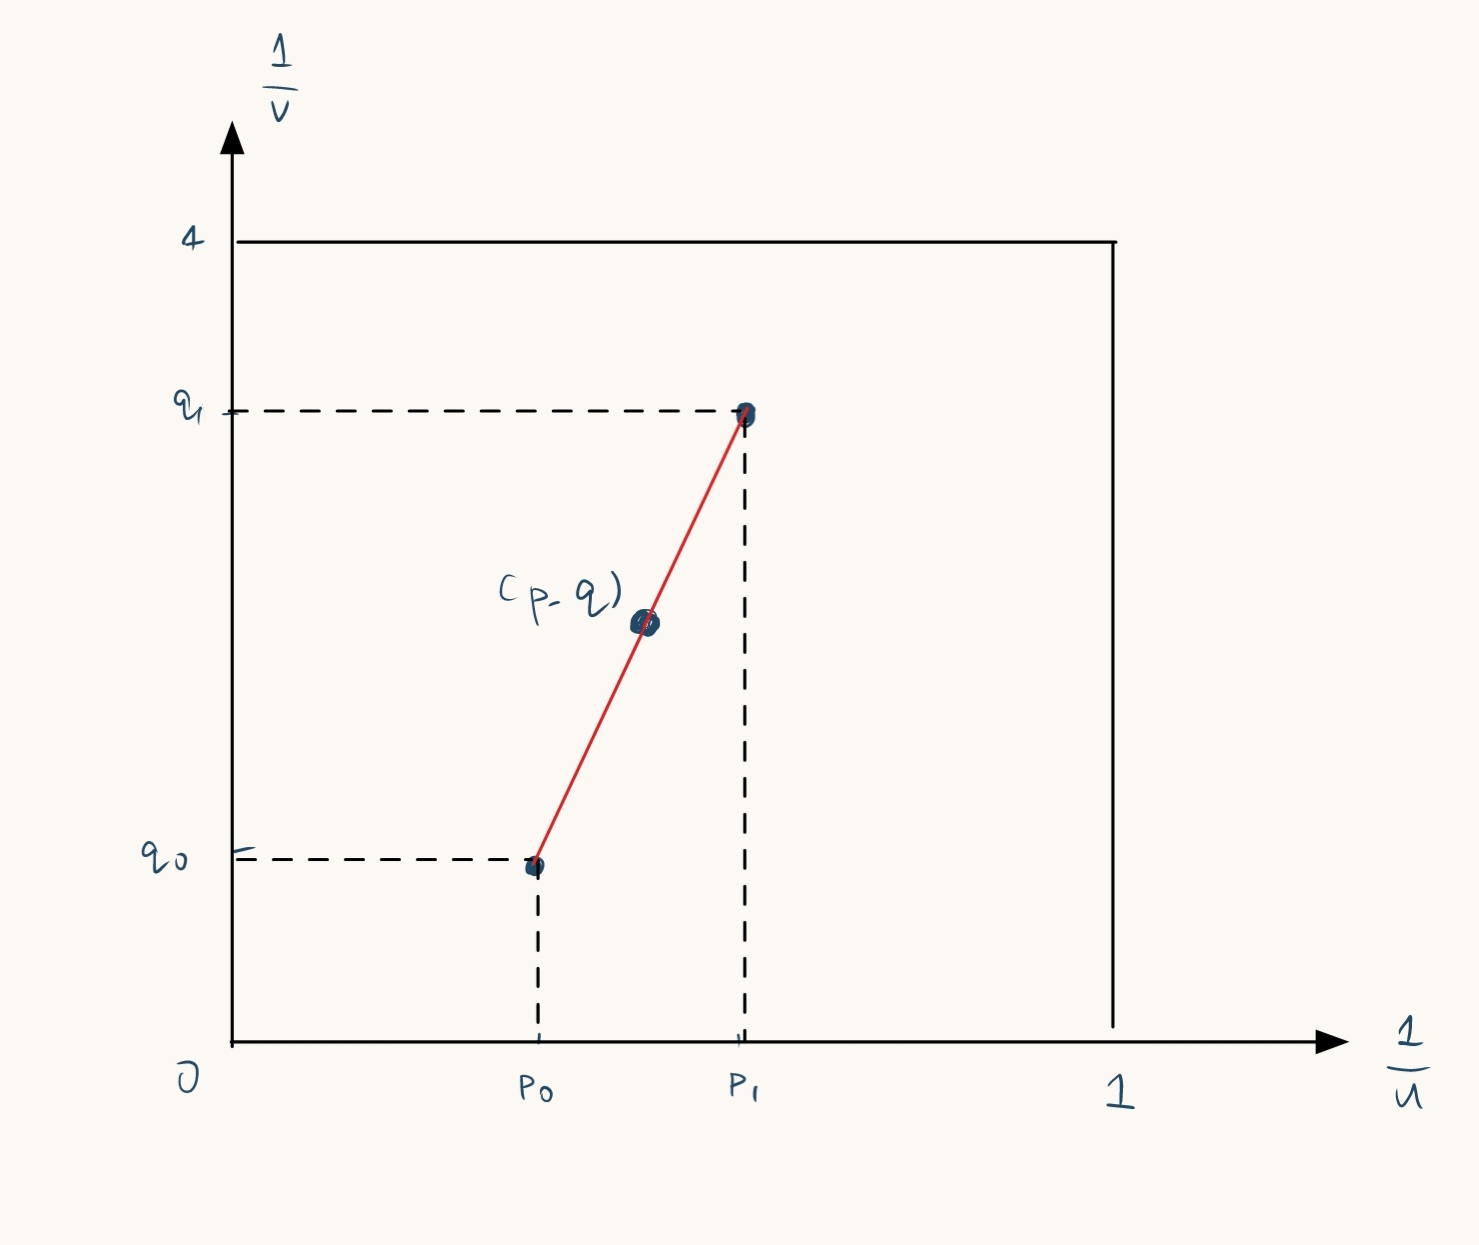
\includegraphics[width=0.5\linewidth]{fig/riesz-thorin-fig.jpg}
    \caption{即对于两点连线之上的任意一点都是有界的}
    \label{fig:Riesz-Thorin}
\end{figure}

且$\forall f\in L^p$,$p_0 < p < p_1$,则$f=f_0+f_1$,其中$f_0\in L^{p_0}$,$f_1\in L^{p_1}$。即
\begin{align*}
    f(x) = f(x)\chi_{ |f(x)| > 1 }(x) + f(x) \chi_{|f(x)| \leqslant 1}
\end{align*}
且
\begin{align*}
    \int |f_0(x)|^{p_0} dx = \int_{\{x: |f(x)| > 1\}} |f(x)|^{p_0} \cdot 1^{p-p_0} dx \leqslant \int_{\mathbb{R}^n} |f(x)|^{p_0} |f(x)|^{p-p_0} dx = \|f\|_p^p < +\infty
\end{align*}

\begin{theorem}[Young Inequation]
    对于$1\leqslant p,q\leqslant +\infty$,则有
    \begin{align*}
        \|f * g\|_r \leqslant \|f\|_p \|g\|_q
    \end{align*}
    其中
    \begin{align*}
        \frac{1}{r} = \frac{1}{p} + \frac{1}{q} - 1
    \end{align*}
\end{theorem}
\begin{proof}
    固定$p$,$q=1$,则
    \begin{align*}
        \eqnmarkbox[red]{1}{\|f * g\|_p \leqslant \|f\|_p \|g\|_1}
    \end{align*}
    我们利用广义的Minkowski Inequation,
    \begin{align*}
        \left\| \int f(x-y) g(y) dy \right\|_p &\leqslant \int_{\mathbb{R}^n} \| f(x-y)\|_p |g(y)| dy \\
        &= \|f\|_p \|g\|_1
    \end{align*}

    $q = p^{\prime}$时,
    \begin{align*}
        \|f * g\|_{\infty} \leqslant \|f\|_p \|g\|_{p^{\prime}} 
    \end{align*}
    即
    \begin{align*}
        \left\| \int f(x-y) g(y) dy \right\|_{\infty} & \leqslant \left\|\int |f(x-y)| |g(y)| dy \right\| \\
        & \overset{\text{Hölder}}{\leqslant} \|f\|_p \|g\|_{p^{\prime}}
    \end{align*}

    而由上述两个点我们可以发现
    \begin{align*}
        \|T g \|_p & \leqslant A_0 \|g\|_1 \\
        \|T g\|_{\infty} &\leqslant A_1 \|g\|_{p^{\prime}}
    \end{align*}
    由Riesz-Thorin Interpolation,$\forall 1< q<p^{\prime}$,有
    \begin{align*}
        \|Tg\|_r \leqslant A_0^{1-\theta} A_1^{\theta} \|g\|_q
    \end{align*}
    其中
    \begin{align*}
        \frac{1}{q} &= \frac{1-\theta}{1} + \frac{\theta}{p^{\prime}} \\
        \frac{1}{r} &= \frac{1-\theta}{p} + \frac{\theta}{\infty}
    \end{align*}
    化简可以得到
    \begin{align*}
        \frac{1}{q} &= \frac{p}{r} + \frac{1}{p^{\prime}} - \frac{p}{rp^{\prime}} \\
        &= \frac{1}{r} - \frac{1}{p^{\prime}} \\
        \frac{1}{r} &= \frac{1}{q} - (1 - \frac{1}{p}) \\
        & = \frac{1}{p} + \frac{1}{q} - 1
    \end{align*}
\end{proof}

\newpage
\section{Fourier积分与求和}
考虑
\begin{align*}
    \lim\limits_{R\to\infty} \int_{B(0,R)} \widehat{f}(\xi) e^{2\pi i x\xi} d\xi \overset{?}{=} f(x)
\end{align*}

\begin{definition}
    $n=1$,定义
    \begin{align*}
        S_R f(x) &= \int\limits_{-R}^R \widehat{f}(\xi) e^{2\pi i x \xi} d\xi, \quad S_R(f) \xrightarrow[L^p]{a.e.} f \\
        & = f * D_R
    \end{align*}
    其中
    \begin{align*}
        D_R(x) = \frac{\sin(2\pi R x)}{\pi x}
    \end{align*}
\end{definition}
\begin{proof}
    \begin{align*}
        S_R f(x) & = \int_{-R}^R \int_{\mathbb{R}} f(y) e^{-2\pi iy \xi} dy e^{2\pi i x \xi} d\xi \\
        & = \int_{\mathbb{R}} f(y) \eqnmarkbox[red]{v1}{\int_{-R}^R e^{-2\pi i (y-x)\xi} d\xi} dy 
 \end{align*}
 \annotate[yshift=-0.5em]{below,right}{v1}{$D_R(y-x)$}

 即
 \begin{align*}
     \int_{-R}^R e^{-2\pi i u \xi} d\xi &= 2\int_0^R \cos(2\pi u \xi) d\xi \\
     & = \frac{2 \sin(2\pi u \xi)}{2\pi u}\bigg|_0^R = \frac{\sin(2\pi u R)}{\pi u}
 \end{align*}

而
\begin{align*}
    \int_{\mathbb{R}} |D_R(x)| dx & = \int_{\mathbb{R}} \frac{|\sin(2\pi R x)|}{|2R\pi x|} d(2Rx) = 2\int_0^{+\infty} \frac{|\sin u|}{|u|} du = +\infty
\end{align*}
因而非绝对收敛,即$D_R\notin L^1$,但$D_R \in L^q$,$\forall q>1$。
\begin{align*}
    \int_{\mathbb{R}} \left| \frac{\sin (2\pi R x)}{\pi x}\right|^q dx = \int_{|x|<1} (2R)dx + \int_{|x|\geqslant 1} \frac{1}{|\pi x|^q}dx < + \infty
\end{align*}
\end{proof}

\begin{theorem}
    当$n=1$,$1<p<\infty$\footnote{\text{Chap3,复杂}},
    \begin{align*}
        \|S_R f\|_p \leqslant C_p \|f\|_p 
    \end{align*}

    $f\in L^p$,$1<p<+\infty$,
\begin{align*}
    S_R f(x) \to f(x) \quad a.e.\ x\in\mathbb{R}
\end{align*}
\end{theorem}

\subsection{求和法}
\subsubsection{算术平均求和法}
定义:
\begin{align*}
    \sigma_R f(x) &\triangleq \frac{1}{R} \int_0^R S_t f(x) dt \\
    & = f * F_R(x)
\end{align*}
其中
\begin{align*}
    F_R(x) & = \left[\frac{\sin (\pi R x)}{\pi x }\right]^2 \frac{1}{R}
\end{align*}
称为Fejer核。
\begin{proof}
    \begin{align*}
        \sigma_R f(x) &= \frac{1}{R} \int_0^R \int_{\mathbb{R}} f(x-y) D_t(y) dy dt \\
        & = \int_{\mathbb{R}} \eqnmarkbox[red]{v3}{\frac{1}{R} \int_0^R D_t(y) dt} f(x-y) dy
    \end{align*}
    \annotate[yshift=-0.5em]{below,right}{v3}{$\triangleq F_R(y)$}

    从而
    \begin{align*}
        F_R(y) &\triangleq \frac{1}{R} \int_0^R \frac{\sin(2\pi t y)}{\pi y} dt \\
        & = -\frac{1}{R} \frac{\cos(2\pi t y)}{2\pi y \cdot \pi y} \\
& = \frac{1- \cos(2\pi R y)}{2R(\pi y)^2}
& = \frac{\sin^2(\pi R y)}{R(\pi y)^2}
    \end{align*}

   且
   \begin{align*}
       \int_{\mathbb{R}} F_R(x) dx & = \int \frac{\sin^2(\pi R x)}{(R\pi x)^2} d(xR) \\
       & = \frac{1}{\pi} \int \frac{\sin^2(\pi u)}{(\pi u)^2} d(\pi u) \\
       & = \frac{1}{\pi} \int_{\mathbb{R}} \frac{\sin^2 t }{t^2} dt = 1
   \end{align*}
\end{proof}

\begin{enumerate}[leftmargin=1cm, label=\arabic*]
    \item $F_R\in L^1$,
    \begin{align*}
        \int_{\mathbb{R}} |F_R(x)| dx = 1
    \end{align*}

    \item $F_R(x) \geqslant 0$,当$f\in L^p$,
    \begin{align*}
        \lim\limits_{R\to+\infty} \| F_R * f - f\|_p = 0
    \end{align*}
    当$f\in C_0$,
    \begin{align*}
        \lim\limits_{R\to +\infty} \|F_R*f - f\|_{\infty} = 0
    \end{align*}
\end{enumerate}

\subsubsection{Abel求和}
\begin{align*}
    \lim\limits_{t\to 0} \int_{\mathbb{R}} e^{-2\pi t |\xi|} \widehat{f}(\xi) e^{2\pi i x \xi} d\xi \overset{?}{=} f(x)
\end{align*}
在$L^p$意义下,或是a.e.意义下。

\paragraph{Poisson积分}
\begin{align*}
    u(x,t) \triangleq \int_{\mathbb{R}} e^{-2\pi t |\xi|} \widehat{f}(\xi) e^{2\pi i x \xi} d\xi = f*P_t
\end{align*}

\paragraph{Gauss积分}
\begin{align*}
    w(x,t) \triangleq \int_{\mathbb{R}} e^{-\pi t^2 |\xi|^2} \widehat{f}(\xi) e^{2\pi i x \xi} d\xi = f * W_t
\end{align*}

\begin{proof}
    \begin{align*}
        w(x,t) & = \int_{\mathbb{R}} e^{-\pi t^2 |\xi|^2} \int f(y) e^{-2\pi i y \xi} dy e^{2\pi i x \xi} d\xi \\
        & = \int_{\mathbb{R}} \eqnmarkbox[red]{v5}{\int_{\mathbb{R}} e^{-\pi t^2 |\xi|^2} e^{-2\pi i \xi(y-x)} d\xi} f(y) dy
    \end{align*}
    \annotate[yshift=-0.5em]{below,right}{v5}{$=W_t(x-y)$}

    已知
    \begin{align*}
        \widehat{e^{-\pi |x|^2}} = e^{-\pi |\xi|^2}
    \end{align*}
    从而
    \begin{align*}
        W_t(u) & = \widehat{\left(e^{-\pi t^2 |\xi|^2} \right)} (-u) \\
        & = \frac{1}{t^n} e^{-\pi \left|\frac{-u}{t}\right|^2} = \frac{1}{t^n} e^{-\pi \frac{u^2}{t^2}}
    \end{align*}
\end{proof}

\begin{enumerate}[leftmargin=1cm, label=\arabic*]
    \item $W_t(u)\in L^1$,$\int W_t(u) du =1$,
    \begin{align*}
        W_t(u) &= (e^{-\pi u^2})_t \quad \psi_t(u) \triangleq \frac{1}{t^n} \psi(\frac{u}{t}) \\
        P_t(u) &= \left(c_n \frac{1}{(1+|x|^2)^{\frac{n+1}{2}}} \right)
    \end{align*}
\end{enumerate}


\paragraph{恒等逼近}
\begin{align*}
    \phi\in L^1(\mathbb{R}),\quad \int_{\mathbb{R}} \phi(x) dx = 1
\end{align*}
定义
\begin{align*}
    \phi_t(x) \triangleq \frac{1}{t^n} \phi\left(\frac{x}{t}\right),\quad \forall t>0,\quad \forall x\in\mathbb{R}^n
\end{align*}

\begin{theorem}
    \begin{enumerate}[leftmargin=1cm, label=\arabic*]
        \item $\forall f\in L^p(\mathbb{R}^n)$,
        \begin{align*}
            \|f*\phi_t - f\|_{p} \to 0, \quad t\to 0 \quad 1\leqslant p\leqslant +\infty
        \end{align*}

        \item $\forall f\in C_0(\mathbb{R}^n)$,(减弱为$f\in UC\footnote{一致连续}\cap L^{\infty}$亦满足)
        \begin{align*}
            \|f * \phi_t - f\|_{\infty} \to 0,\quad \text{when}\ t\to 0
        \end{align*}
    \end{enumerate}
\end{theorem}
\begin{proof}
    \begin{align*}
        \| f*\phi_t(x) - f(x) \cdot 1\|_p & = \left\| \int f(x-y)\phi_t(y) dy - \int f(x)\phi_t(y) dy \right\| \\
        &= \left\|\int_{\mathbb{R}^n} [f(x-y) - f(x)] \phi_t(y) dy \right\| \\
        & \overset{\texttt{Minkowski}}{\leqslant} \int_{|y|<\delta} + \int_{|y|\geqslant \delta} \\
        & < \varepsilon \int_{\mathbb{R}^n} |\phi_t(y)|dy + 2\|f\|_p \int_{|y|\geqslant \delta} |\phi_t(y)| dy \\
        & < \varepsilon \int_{\mathbb{R}^n} |\phi_t(y)|dy + 2\|f\|_p \int_{|y|\geqslant \delta} \frac{1}{t^n} \phi\left(\frac{y}{t}\right) dy < \varepsilon^{\prime}
    \end{align*}
\end{proof}

% 10th, Oct
\chapter{Hardy-Littlewood极大算子}
\section{恒等逼近}
$\phi\in L^1(\mathbb{R}^n)$,$\int_{\mathbb{R}^n} \phi(x) dx = 1$,$\forall t > 0$,定义:
\begin{align*}
    \phi_t(x) \triangleq \frac{1}{t^n} \phi\left(\frac{x}{t}\right)
\end{align*}

\begin{Corollary}
    \begin{enumerate}[leftmargin=1cm, label=\arabic*.]
        \item 
        \begin{align*}
            \|f * F_{\frac{1}{R}} - f\|_p \to 0
        \end{align*}
        其中$F$为Fejer Kernel
        \begin{align*}
            F_{\frac{1}{R}} \triangleq \frac{\sin^2(\pi R x)}{(\pi x)^2 R} = \left(\frac{\sin^2(\pi u)}{(\pi u)^2}\right)_{\frac{1}{R}}
        \end{align*}

        \item 
        \begin{align*}
            \|f * P_t - f\|_p \to 0
        \end{align*}
        其中$P$为Poisson Kernel
        \begin{align*}
            P_t = \left( c_n \frac{1}{(1 + |x|^2)^{\frac{n+1}{2}}} \right)_t
        \end{align*}

        \item 
        \begin{align*}
            \|f*W_t - f\|_p \to 0
        \end{align*}
        其中$W$为Gauss Kernel
        \begin{align*}
            W_t = \left(e^{-\pi^2 |x|^2} \right)_t
        \end{align*}
    \end{enumerate}
\end{Corollary}

\begin{Corollary}
    \begin{align*}
        \phi_t \xrightarrow{\mathcal{S}^{\prime}}\ \delta,\quad \text{when}\ t\to 0
    \end{align*}
    即$\forall \phi\in \mathcal{S}(\mathbb{R}^n)$,$\int \phi_t(x) \psi(x) dx \to \psi(0)$,当$t\to 0$。
\end{Corollary}
    
\paragraph{Question} 当$f\in L^p(\mathbb{R}^n)$,$1\leqslant p< \infty$,
\begin{align*}
    \left.\begin{array}{c}
        f*F_{\frac{1}{R}} \\
        f*W_t \\
        f*P_t
    \end{array} \right\rbrace \xrightarrow[?]{a.e.} \ f(x)
\end{align*}

上述问题等价于$\lim\limits_{R\to\infty} f*F_{\frac{1}{R}}$存在a.e.

\section{点态收敛与极大算子的有界性}
\begin{definition}[次线性算子]
    若$T$为次线性算子,当且仅当:
    \begin{enumerate}[leftmargin=1cm, label=\arabic*.]
        \item $|T(f+g)(x)| \leqslant |Tf(x)| + |Tg(x)|$;
        \item $|T(cf)(x)| = |c|\cdot |Tf(x)|$,$\forall c\in \mathbb{C}$。
    \end{enumerate}
\end{definition}

\begin{definition}[强$p,q$型]
    $T$称为强$p,q$型算子,当且仅当$\|Tf\|_q \leqslant C_{p,q} \|f\|_p$,$\forall f\in L^p$,$0<p,q<\infty$。
\end{definition}

\begin{definition}[弱$p,q$型]
    $T$称为弱$p,q$型算子,当且仅当$|\{x: |Tf(x)| > \lambda\}| \leqslant \left( \frac{c\|f\|_p}{\lambda}\right)^q$,$\forall f\in L^p$,$0<p,q<\infty$。
\end{definition}

\begin{Corollary}
    强$p,q$显然可以推出弱$p,q$型:
    \begin{align*}
        \left(\int_{\mathbb{R}^n} |Tf(x)|^q dx \right)^{\frac{1}{q}} \leqslant C_{p,q} \|f\|_p
    \end{align*}
\end{Corollary}
\begin{proof}
    考虑左侧放缩
    \begin{align*}
        \operatorname{LHS} \geqslant \left(\int_{\{x: |Tf(x)| > \lambda\}}  |Tf(x)|^q dx \right)^{\frac{1}{q}} \geqslant \left(\int_{\{x: |Tf(x)| > \lambda\}}  \lambda^q dx \right)^{\frac{1}{q}}  \geqslant \lambda \cdot \left|\{x: |Tf(x)| > \lambda \}\right|^{\frac{1}{q}}
    \end{align*}

    因此有
    \begin{align*}
        \left|\{x: |Tf(x)| > \lambda \}\right|^{\frac{1}{q}} \leqslant \frac{C_{p,q}\|f\|_p}{\lambda}
    \end{align*}
    即得
\end{proof}
    
\begin{Corollary}
    将空间改为测度空间依然满足,即$(\mathscr{X},\mu)$,其中$\mu$为测度,满足
    \begin{enumerate}[leftmargin=1cm, label=\arabic*.]
        \item $\mu(\varnothing) = 0$;
        \item $0\leqslant \mu(E) \leqslant +\infty$;
        \item $\mu(\bigcup\limits_{i=1}^{\infty} E_i) = \sum\limits_{i=1}^{\infty} \mu(E_i)$
    \end{enumerate}
\end{Corollary}

\begin{theorem}
    $\forall t\in I$,$T_t$为$L^p(\mathscr{X},\mu)\to L^q(\mathscr{Y},\nu)$的一个可测函数空间,$T_t$为线性算子,定义极大算子
    \begin{align*}
        T^* (f)(x) \triangleq \sup\limits_{t\in I} |T_t(f)(x)|
    \end{align*}
    若$T^*$为弱$p,q$型,设$t_0\in \overline{I}$,则
    \begin{align*}
        \mathcal{F} \triangleq \{f\in L^p(\mathscr{X},\mu): \lim\limits_{t\to t_0} T_t f(x) = f(x),\ a.e.\ x\in\mathscr{X} \}
    \end{align*}
    为$L^p(\mathscr{X},\mu)$的闭集。
\end{theorem}
\begin{proof}
    设$f_n\in\mathcal{F}$,且$f_n\xrightarrow{L^p}\ f$,往证$f\in\mathcal{F}$\footnote{为了证明$\forall f\in L^p$,
    \begin{align*}
        \lim\limits_{t\to t_0} T_t f(x) = f(x)\ a.e.
    \end{align*}
    只需
    \begin{enumerate}[leftmargin=1cm, label=\arabic*.]
        \item $\forall f\in C_0^{\infty}$;
        \item $\sup\limits_{t>0} |T_t f(x)|$为弱$p,q$型。
    \end{enumerate}},即意味着该集合的聚点都在集合内,即为闭集。

    而$f\in L^p$,显然。因此我们往证
    \begin{align*}
        \lim\limits_{t\to t_0} |T_t f(x) - f(x)| = 0 \quad a.e.
    \end{align*}
    即
    \begin{align*}
        \mu\left\lbrace\overline{\lim\limits_{t\to t_0}} |T_t f(x) - f(x)| > 0 \right\rbrace = 0 
    \end{align*}
    即$\forall \lambda>0$,
    \begin{align*}
        \mu\left\lbrace x\in\mathscr{X}:\  \overline{\lim\limits_{t\to t_0}} |T_t f(x) - f(x)| >  \lambda \right\rbrace = 0 
    \end{align*}

    而
    \begin{align*}
        \overline{\lim\limits_{t\to t_0}} |T_t f(x) - f(x)| &= \overline{\lim\limits_{t\to t_0}} |T_t f(x) - T_t f_n(x) + T_t f_n(x) - f_n(x) + f_n(x) - f(x) | \\
        & \leqslant \overline{\lim\limits_{t\to t_0}} |T_t(f-f_n)(x)| + \overline{\lim\limits_{t\to t_0}} |T_tf_n(x) - f_n(x)| + |f_n(x) - f(x)| 
    \end{align*}

    故而
    \begin{align*}
        \left\lbrace x\in\mathscr{X}:\ \overline{\lim\limits_{t\to t_0}} |T_tf(x) - f(x)| > \lambda\right\rbrace \subseteq \left\lbrace x\in\mathscr{X}:\ \overline{\lim\limits_{t\to t_0}} |T_t(f- f_n)| + \overline{\lim\limits_{t\to t_0}} |T_tf_n -f_n| + |f_n - f| > \lambda \right\rbrace
    \end{align*}
    即
    \begin{align*}
        \operatorname{LHS} = \mu\left\lbrace x\in\mathscr{X}:\ \overline{\lim\limits_{t\to t_0}} |T_tf(x) - f(x)| > \lambda\right\rbrace \leqslant  \mu \left\lbrace x\in\mathscr{X}:\ \overline{\lim\limits_{t\to t_0}} |T_t(f- f_n)| + \overline{\lim\limits_{t\to t_0}} |T_tf_n -f_n| + |f_n - f| > \lambda \right\rbrace
    \end{align*}

    记$E_n = \left\lbrace x\in \mathscr{X}:\ \overline{\lim\limits_{t\to t_0}} T_t f_n(x) \neq f_n(x)\right\rbrace$,$E\triangleq\bigcup\limits_{n=1}^{\infty} E_n$,$\mu(E)=0$。

    从而
    \begin{align*}
        \operatorname{LHS} &\leqslant \mu\left\lbrace x\in\mathscr{X}:\ \overline{\lim\limits_{t\to t_0}} |T_tf(x) - T_tf_n(x)| > \frac{\lambda}{2} \right\rbrace + \mu\left\lbrace x\in\mathscr{X}:\ \overline{\lim\limits_{t\to t_0}} |f_n(x) - f(x)| > \frac{\lambda}{2} \right\rbrace \\
        & \leqslant \left( \frac{c \|f-f_n\|_p}{\frac{\lambda}{2}}\right)^q + \left( \frac{c \|f-f_n\|_p}{\frac{\lambda}{2}}\right)^p \to 0
    \end{align*}
\end{proof}

\begin{theorem}
    条件同theorem 2.2.1,则
    \begin{align*}
        \widetilde{\mathcal{F}} \triangleq \left\lbrace f\in L^p(\mathscr{X},\mu)\  \lim\limits_{t\to 0} T_t f(x)\ a.e.\ \text{存在}\right\rbrace
    \end{align*}
    $\widetilde{\mathcal{F}}$在$L^p(\mathscr{X},\mu)$中为闭集。
\end{theorem}
\begin{proof}
    设$f_n\in\widetilde{\mathcal{F}}$,$f_n\to f$,往证$f\in\widetilde{\mathcal{F}}$。只需证明$\forall \lambda>0$,
    \begin{align*}
        \mu\left\lbrace x\in\mathscr{X}: \ \overline{\lim\limits_{t\to t_0}} T_tf(x) - \varliminf\limits_{t\to t_0} T_t f(x) > \lambda\right\rbrace = 0
    \end{align*}
    \textcolor{red}{即上下极限之差几乎处处为$0$,当然这里不需要加绝对值,则充要条件即为$\lim\limits_{t\to t_0} T_t f(x)$几乎处处存在。由于其为线性算子,则这个条件就等价于在$0$处极限几乎处处存在,这个充要性是在泛函分析中提及的。}记$\Omega(f)(x)\triangleq \varlimsup\limits_{t\to t_0}T_tf(x) - \varliminf\limits_{t\to t_0} T_t f(x)$,则显而易见的有
    \begin{align*}
        \color{red} \Omega(f)(x) \leqslant 2T^*(f)(x)
    \end{align*}
    并且有
    \begin{enumerate}[leftmargin=1cm, label=\arabic*.]
        \item $\Omega(f) \geqslant 0$;
        \item $\Omega(f+g) \leqslant \Omega(f) + \Omega(g)$\footnote{\begin{align*}
            \varlimsup\limits_{t\to t_0}T_t(f+g)(x) - \varliminf\limits_{t\to t_0} T_t (f+g)(x) &= \varlimsup\limits_{t\to t_0} (T_t f + T_t g) - \varliminf\limits_{t\to t_0} (T_t f + T_t g) \\
            & \left[\leqslant \varlimsup\limits_{t\to t_0}  T_t f + \varlimsup\limits_{t\to t_0} T_t g \right]- \left[\varliminf\limits_{t\to t_0} T_t f + \varliminf\limits_{t\to t_0} T_t g\right] \\
            & = \Omega(f) + \Omega(g)
        \end{align*}};
    \end{enumerate}

    \begin{align*}
        \mu\{x\in\mathscr{X}:\ \Omega(f)(x) > \lambda\} &\leqslant \mu  \{ x\in\mathscr{X}:\ \Omega(f-f_n) + \Omega(f_n) > \lambda \} \\
        & \leqslant \mu \{x\in\mathscr{X}:\ \Omega(f-f_n) > \frac{\lambda}{2} \} + \mu \{x\in\mathscr{X}:\ \Omega(f_n) > \frac{\lambda}{2} \} \\
        & \leqslant \mu \{x\in\mathscr{X}:\ 2T^*(f-f_n)(x) > \frac{\lambda}{2} \} + (\to 0) \leqslant \left(\frac{c\|f-f_n\|_p}{\frac{\lambda}{4}}\right)^q + (\to 0) \to 0
    \end{align*}
\end{proof}

% 15th Oct
\newpage
\section{Marcinkiewicz内插定理}
\begin{lemma}
    $\forall\ 0<p<\infty$,
    \begin{align*}
        \|f\|_{p}^p = \int_0^{\infty} p \lambda^{p-1} \bigg|\{x\in\mathbb{R}^n:\ |f(x)| > \lambda\}\bigg| d\lambda
    \end{align*}
\end{lemma}
\begin{proof}
    \begin{align*}
        \operatorname{RHS} &= \int_0^{\infty} p \lambda^{p-1} \int_{\mathbb{R}^n} \chi_{x: |f(x)|>\lambda}(x) dx d\lambda \\
        & \overset{\texttt{Tonelli}}{=} \int_{\mathbb{R}^n} \int_0^{|f(x)|} p\lambda^{p-1}  d\lambda dx \\
        & = \int_{\mathbb{R}^n} \lambda^p\bigg|_{0}^{|f(x)|} dx \\
        & = \int_{\mathbb{R}^n} |f(x)|^p dx = \|f\|_p^p
    \end{align*}
\end{proof}

\begin{lemma}
    若$f\in L^p(\mathbb{R}^n)$,$0<p_0<p<p_1\leqslant\infty$,则
    \begin{align*}
        f = f_0 + f_1 \quad f_0\in L^{p_0}, \quad f_1\in L^{p_1}
    \end{align*}
\end{lemma}
\begin{proof}
    令
    \begin{align*}
        f_0(x) &= f(x) \chi_{\{|f(x)| > 1\}} (x) \\
        f_1(x) &= f(x) \chi_{\{|f(x)| \leqslant 1\}} (x)
    \end{align*}
    而后交换次序即可得到$f_i\in L^{p_i}$,$i=0,1$。
\end{proof}

\begin{theorem}[Marcinkiewicz interpolation]
    $\forall 1\leqslant p_0 < p_1 \leqslant \infty$,$T$为$L^{p_0} + L^{p_1} \to L^{p_0} + L^{p_1}$为次线性算子,
    \begin{enumerate}[leftmargin=1cm, label=\arabic*.]
        \item $T$是弱$(p_0,p_0)$型:
        \begin{align*}
        \left| \{ x\in\mathbb{R}^n :\ |Tf(x)| > \lambda\} \right| \leqslant \left(\frac{c_0 \|f\|_{p_0}}{\lambda}\right)^{p_0}
        \end{align*}
        \item $T$是弱$(p_1, p_1)$型:
        \begin{align*}
            \left| \{ x\in\mathbb{R}^n :\ |Tf(x)| > \lambda\} \right| \leqslant \left(\frac{c_1 \|f\|_{p_1}}{\lambda}\right)^{p_1}
        \end{align*}
    \end{enumerate}
    则$\forall p_0 < p < p_1$,有$T$是强$(p,p)$型,即
    \begin{align*}
        \|Tf\|_{p} \leqslant 2 p^{\frac{1}{p}} c_0^{1-\theta} c_1^{\theta} \left( \frac{1}{p-p_0} + \frac{1}{p_1 - p} \right)^{\frac{1}{p}} \|f\|, \quad \frac{1}{p} = \frac{1-\theta}{p_0} + \frac{\theta}{p_1},\quad \text{where}\ 0<\theta<1
    \end{align*}
    
    可推广至下三角。
\end{theorem}
\begin{proof}
    先证明$p_1<\infty$的情形,$f\in L^p$
    \begin{align*}
        \|Tf\|_p^p &= p\int_0^{\infty} \lambda^{p-1} |\{x:\ |Tf(x)| > \lambda \}| d\lambda 
    \end{align*}
    令
    \begin{align*}
        f_0^{\lambda}(x) &= f(x) \chi_{\{x: |f(x)| > \alpha\lambda \}} \\
        f_1^{\lambda}(x) &= f(x) \chi_{\{x: |f(x)| \leqslant \alpha\lambda \}}
    \end{align*}
    其中$\alpha>0$待定,则
    \begin{align*}
        \mu|\underbrace{\{x:\ |Tf(x)| > \lambda \}}\limits_{E}| &\overset{\textit{次线性}}{\leqslant} \mu\{x: |Tf_0^{\lambda}| + |Tf_1^{\lambda}| > \lambda \} \\
        & \mu|\underbrace{\left\lbrace x: |Tf_0^{\lambda}| > \frac{\lambda}{2}\right\rbrace }\limits_{E_1}| + \mu|\underbrace{\left\lbrace x: |Tf_1^{\lambda}| > \frac{\lambda}{2}\right\rbrace }\limits_{E_2}|
    \end{align*}
    这是由于$E\subseteq E_1\cup E_2$。故而
    \begin{align*}
        \|Tf\|_p^p &\leqslant \underbrace{p \int_0^{\infty} \lambda^{p-1} \left(  \frac{c_0 \|f\|_{p_0}}{\frac{\lambda}{2}}\right)^{p_0} d\lambda}\limits_{I_0} + \underbrace{p \int_0^{\infty} \lambda^{p-1} \left(  \frac{c_1 \|f\|_{p_1}}{\frac{\lambda}{2}}\right)^{p_1} d\lambda}\limits_{I_1} 
    \end{align*}
    而
    \begin{align*}
        I_0 & = p c_0^{p_0} 2^{p_0} \int_0^{\infty} \lambda^{p-1-p_0} \int_{\mathbb{R}^n} |f_0^{\lambda}(x)|^{p_0} dx d\lambda \\
        & = p (2c_0)^{p_0} \int_0^{\infty} \lambda^{p-1-p_0} \int_{\{|f(x)| > \alpha\lambda \}} |f(x)|^{p_0} dxd\lambda \\
        & \overset{\texttt{Tonelli}}{=} p(2c_0)^{p_0} \int_{\mathbb{R}^n} \int_0^{\frac{|f(x)|}{\alpha}} \lambda^{p-1-p_0} |f(x)|^{p_0} d\lambda dx \\
        & = p(2c_0)^{p_0} \int_{\mathbb{R}^n} \frac{\lambda^{p-p_0}}{p-p_0}\bigg|_{0}^{\frac{|f(x)|}{\alpha}} |f(x)|^{p_0} dx \\
        & = \underbrace{p(2c_0)^{p_0} \frac{1}{p-p_0} \frac{1}{\alpha^{p-p_0}}}\limits_{C(p)} \int_{\mathbb{R}^n} |f(x)|^p dx
    \end{align*}

    第二部分
    \begin{align*}
        I_1 & = p (2c_1)^{p_1} \int_0^{\infty} \int_0^{\infty} \lambda^{p-1-p_1} \int_{\mathbb{R}^n} |f_1^{\lambda}(x)|^{p_1} dx d\lambda \\
        & = p (2c_1)^{p_1} \int_0^{\infty} \lambda^{p-1-p_1} \int_{\{|f(x)| \leqslant \alpha\lambda \}} |f(x)|^{p_1} dxd\lambda \\
        & \overset{\texttt{Tonelli}}{=} p(2c_0)^{p_0} \int_{\mathbb{R}^n} \int_{\frac{|f(x)|}{\alpha}}^{\infty} \lambda^{p-1-p_1} |f(x)|^{p_1} d\lambda dx \\
        & = p(2c_1)^{p_1} \int_{\mathbb{R}^n} \frac{\lambda^{p-p_1}}{p-p_1}\bigg|_{\frac{|f(x)|}{\alpha}}^{\infty} |f(x)|^{p_1} dx \\
        & = p(2c_1)^{p_1} \frac{1}{p_1 - p} \frac{1}{\alpha^{p-p_1}} \int_{\mathbb{R}^n} |f(x)|^p dx
    \end{align*}

    因此
    \begin{align*}
        \|Tf\|_p^p &\leqslant p (2c_0)^{p_0} \frac{1}{\alpha^{p-p_0}} \frac{1}{p-p_0} \|f\|_p + p(2c_1)^{p_1} \frac{1}{\alpha^{p-p_1}} \frac{1}{p_1-p} \|f\|_p^p \\
        & = p \|f\|_p^p \left[\frac{(2c_0)^{p_0}}{\alpha^{p-p_0}} \frac{1}{p-p_0} + \frac{(2c_1)^{p_1}}{\alpha^{p-p_1}}\frac{1}{p_1-p} \right]
    \end{align*}

    我们要选择$\alpha$,使得
    \begin{align*}
        \frac{(2c_0)^{p_0}}{\alpha^{p-p_0}} = \frac{(2c_1)^{p_1}}{\alpha^{p-p_1}} \triangleq M
    \end{align*}
    即就是
    \begin{align*}
        \alpha \triangleq \left[ \frac{(2c_0)^{p_0}}{(2c_1)^{p_1}} \right]^{\frac{1}{p_1 - p_0}}
    \end{align*}

    因此
    \begin{align*}
        \frac{(2c_0)^{p_0}}{\alpha^{p-p_0}} &= (2c_0)^{p_0} \left[ \frac{(2c_1)^{p_1}}{(2c_0)^{p_0}} \right]^{\frac{p-p_0}{p_1 - p_0}} \\
        & = (2c_0)^{p_0\left(1 - \frac{p - p_0}{p_1 - p_0}\right)} (2c_1)^{p_1 \frac{p - p_0}{p_1 - p_0}} 
    \end{align*}

    而
    \begin{align*}
        p_0 \frac{p_1 - p}{p_1 - p_0} &= p_0 \frac{1 - \frac{p}{p_1}}{1 -\frac{p_0}{p_1}} = \left[\frac{\frac{1}{p} - \frac{1}{p_1} }{\frac{1}{p_0} - \frac{1}{p_1}}\right] p
    \end{align*}
    而
    \begin{align*}
        \frac{1}{p} = \frac{1- \theta}{p_0} + \frac{\theta}{p_1}
    \end{align*}
    则上式
    \begin{align*}
        \frac{1}{p} &= \frac{1}{p_0} + \left(\frac{1}{p_1} - \frac{1}{p_0}\right)\theta \Rightarrow \\
        \theta &= \frac{\frac{1}{p} - \frac{1}{p_0}}{\frac{1}{p_1} - \frac{1}{p_0}} \\
        1 - \theta & = \frac{\frac{1}{p_1} - \frac{1}{p_0}}{\frac{1}{p_1} - \frac{1}{p_0}}
    \end{align*}

    因此得到
    \begin{align*}
        \|Tf\|_{p} &\leqslant p^{\frac{1}{p}} \|f\|_p \left[(2c_0)^{p\theta} (2c_1)^{p(1-\theta} \left(\frac{1}{p-p_0} + \frac{1}{p_1 - p} \right)\right]^{\frac{1}{p}} \\
        & \leqslant 2 p^{\frac{1}{p}} c_0^{1-\theta} c_1^{\theta} \left( \frac{1}{p-p_0} + \frac{1}{p_1 - p} \right)^{\frac{1}{p}} \|f\|_p, \quad \frac{1}{p} = \frac{1-\theta}{p_0} + \frac{\theta}{p_1},\quad \text{where}\ 0<\theta<1
    \end{align*}

    而对于无穷时候的情况
    \begin{align*}
        \|Tf\|_{\infty} \leqslant c_1 \|f\|_{\infty}
    \end{align*}
    
\end{proof}

\begin{exercise}[Homework 15th Oct]
    证明更一般的Marcinkiewicz内插定理:
    \begin{theorem}[Normal Marcinkiewicz Interpolation]
        若满足
        \begin{enumerate}[leftmargin=1cm, label=\arabic*.]
        \item $T$是弱$(p_0,q_0)$型,$q_0 \geqslant p_0$;
        \item $T$是弱$(p_1, q_1)$型,$q_1\geqslant p_1$,且$q_0\neq q_1$;
    \end{enumerate}
    则$T$是强$(p,q)$型,$p_0<p<p_1$,$q_0<q<q_1$,且
    \begin{align*}
        \frac{1}{p} &= \frac{1-\theta}{p_0} + \frac{\theta}{p_1} \\
        \frac{1}{q} &= \frac{1-\theta}{q_0} + \frac{\theta}{q_1} \\
        \text{where}\ & 0<\theta < 1
    \end{align*}
    \end{theorem}
\end{exercise}
\begin{proof}
    
\end{proof}












\paragraph{Question} 当$\varphi\in L^1(\mathbb{R})$,$\int_{\mathbb{R}^n} \varphi(x) dx = 1$,问:
\begin{align*}
    &f\in L^p ,\ 1\leqslant p<\infty \\
    & \lim\limits_{t\to 0} \varphi_t * f(x) \overset{?}{=} f(x),\ a.e.
\end{align*}

归结于:
\begin{enumerate}[leftmargin=1cm, label=\arabic*.]
    \item 当$f\in C_0^{\infty}$,已证明。
    \item 
    \begin{align*}
        \sup\limits_{t>0} |\varphi_t * f(x)|
    \end{align*}
    是否为弱$(p,q)$型?
\end{enumerate}






\newpage
\section{Hardy-Littlewood极大算子 $\mathcal{M}(f)$}
\begin{definition}[Hardy-Littlewood极大算子]
    $f\in L^1_{\texttt{Loc}} (\mathbb{R}^n)$,定义
    \begin{align*}
        \mathcal{M}f(x) \triangleq \sup\limits_{x\in B} \frac{1}{|B|} \int_{B} |f(y)| dy
    \end{align*}
    其中$B$为$\mathbb{R}^n$中的球。

    也可以以方体定义:
    \begin{align*}
        \mathcal{M}^{\texttt{Cube}}f(x) \triangleq \sup\limits_{x\in Q} \frac{1}{|Q|} \int_{Q} |f(y)| dy
    \end{align*}
    其中$Q$为$\mathbb{R}^n$中平行于坐标面的方体。

    同理,定义
    \begin{align*}
        \widetilde{\mathcal{M}}f(x) \triangleq \sup\limits_{r>0} \frac{1}{|B(x,r)|} \int_{B(x,r)} |f(y)| dy
    \end{align*}
    也可以定义
    \begin{align*}
        \widetilde{\mathcal{M}}^{\texttt{Cube}}f(x) \triangleq \sup\limits_{r>0} \frac{1}{|Q(x,r)|} \int_{Q(x,r)} |f(y)| dy
    \end{align*}
    其中$Q(x,r)$表示以$x$为心,$r$为边长的平行于坐标面的方体。
\end{definition}
\begin{remark}
    自然的,我们可以发现,
    \begin{align*}
        C_2(n) \mathcal{M}^{\texttt{Cube}} f(x) \leqslant \mathcal{M}f(x) \leqslant C_1(n) \mathcal{M}^{\texttt{Cube}} f(x)
    \end{align*}

    这里局部$L^1$与$L^1$不同,例如
    \begin{align*}
        \frac{1}{\sqrt{x}} &\notin L^1(\mathbb{R}) \\
        \frac{1}{\sqrt{x}} &\in L^1_{\texttt{Loc}}(\mathbb{R})
    \end{align*}
    而$x^3 + 5x^2 + 6$也同上有这样的情况。
\end{remark}
\begin{remark}
    自然的我们也可以发现
    \begin{align*}
        \widetilde{\mathcal{M}}f(x) \leqslant \mathcal{M}f(x) \leqslant 2^n \widetilde{M}f(x)
    \end{align*}
\end{remark}
\begin{proof}
    $\forall x\in\mathbb{R}^n$,$\forall x\in B$,$r(B) = r$,则有
    \begin{align*}
        \frac{1}{|B|} \int_B |f(y)| dy \leqslant \frac{1}{|B|} \int_{B(x,2r)} |f(y)| dy = \frac{|B(x,2r)|}{|B|} \frac{1}{|B(x,2r)|} \int_{B(x,2r)} |f(y)| dy \leqslant 2^n \widetilde{\mathcal{M}} f(x)
    \end{align*}
\end{proof}

\begin{proposition}[一个平凡的性质]
    $\mathcal{M}$是强$(\infty,\infty)$型的,更精确地,
    \begin{align*}
        \|Mf\|_{\infty} \leqslant \|f\|_{\infty}
    \end{align*}
\end{proposition}
\begin{proof}
    \begin{align*}
        \mathcal{M}f(x) \triangleq \sup\limits_{x\in B} \frac{1}{|B|} \int_{B} |f(y)| dy \leqslant  \sup\limits_{x\in B} \frac{1}{|B|} \int_{B} \|f\|_{\infty} dy = \|f\|_{\infty}
    \end{align*}
    \textcolor{red}{由于$\infty$-范数的定义为:设 $(\Omega, \mathscr{B}, \mu)$是一个测度空间, $\mu$对于 $\Omega$ 是 $\sigma$-有限的,$u(x)$是$\Omega$上的可测函数。如果$u(x)$与$\Omega$上的一个有界函数几乎处处相等,则称$u(x)$是$\Omega$ 上的一个本性有界可测函数。$\Omega$上的一切本性有界可测函数(把a.e.相等的两个函数视为同一个向量)的全体记作 $L^{\infty}(\Omega, \mu)$,在其上规定:}
    \begin{align*}
        \color{red} \|u\|=\inf _{\substack{\mu\left(E_0\right)=0 \\ E_0 \subset \Omega}}\left(\sup _{x \in \Omega \backslash E_0}|u(x)|\right)
    \end{align*}
    \textcolor{red}{此式右端有时也记作$\underset{x\in\Omega}{\operatorname{ess} \sup}|u(x)|$ 或 $\underset{x\in\Omega}{\operatorname{l.u.b}}|u(x)|$。}
\end{proof}

\begin{proposition}
    $\mathcal{M}f$不是强$(1,1)$的。更确切地,若$f\in L^1$,且$f\neq 0$(不是几乎处处为0),则$\|\mathcal{M}f\|_1 = +\infty$。
\end{proposition}
\begin{proof}
    $f\neq 0$,故而$\exists R>0$,$\exists \varepsilon_0>0$,s.t.
    \begin{align*}
        \int_{B(0,R)} |f(x)| dx \geqslant \varepsilon_0
    \end{align*}

    则$\forall x\in \mathbb{R}^n$,$|x|>R$,则$B(0,R)\subseteq B(x,2|x|)$。我们记
    \begin{align*}
        \bbint |f(y)| dy \triangleq \frac{1}{|B|} \int_B |f(y)| dy
    \end{align*}

    则
    \textcolor{red}{\begin{align*} 
        \mathcal{M}f(x) &\triangleq \sup\limits_{x\in B} \int_B |f(y)| dy \geqslant \frac{1}{|B(x,2|x|)|} \epsilon_0 \\
        & = \frac{\varepsilon_0}{c_n(2|x|)^n} = c' \frac{1}{|x|^n}
    \end{align*}}
    因此当$x\to 0$时,$\mathcal{M}f$将会发散,即
    \begin{align*}
        \|\mathcal{M}f\|_{1} = +\infty
    \end{align*}
\end{proof}

\begin{theorem}
    $\mathcal{M}f$是弱$(1,1)$的,即$\exists c>0$,$\forall \lambda>0$,有
    \begin{align*}
        \left|\underbrace{\left\lbrace x\in\mathbb{R}^n: \mathcal{M}f(x) > \lambda \right\rbrace}\limits_{E_{\lambda}}\right| \leqslant \frac{5^n}{\lambda} \|f\|_1
    \end{align*}
\end{theorem}
\begin{proof}
    若我们先承认Vitali引理(\ref{Th:Vitali}),$\forall x\in E_{\lambda}$,则
    \begin{align*}
        \mathcal{M}f(x) > \lambda
    \end{align*}
    即
    \begin{align*}
        \sup\limits_{x\in B} \bbint_{B} |f(y)| dy > \lambda
    \end{align*}
    则$\exists B^x$,s.t. $x\in B^x$,且
    \begin{align*}
        \frac{1}{|B^x|}\int_{B^x} |f(y)| dy > \lambda
    \end{align*}
    即
    \begin{align*}
        |B^x| < \frac{1}{\lambda} \int_{B^x} |f(y)| dy
    \end{align*}
    从而
    \begin{align*}
        E_{\lambda} \subset \bigcup\limits_{x\in E_{\lambda}} B^x
    \end{align*}
    故而
    \begin{align*}
        |B^x| \leqslant \frac{1}{\lambda} \int_{\mathbb{R}^n} |f(y)| dy = \frac{\|f\|_1}{\lambda}
    \end{align*}
    故而$r(B^{\alpha}) \leqslant \left(\frac{\|f\|_1}{c_n \lambda}\right)^{1/n}$,$\forall x\in E_{\lambda}$,因此由Vitali引理,存在$\{x_j\}_{x_j\in E_{\lambda}}$,s.t.
    \begin{align*}
        B^{x_j} &\cap B^{x_{j'}} = \varnothing,\quad j\neq j' \\
        |E_{\lambda}| &\leqslant 5^n \sum\limits_{j=1}^{\infty} |B^{x_j}| \leqslant 5^n \sum\limits_{j=1}^{\infty} \frac{1}{\lambda} \int_{B^{x_j}} |f(y)| dy \\
        & = \frac{5^n}{\lambda} \sum_{j=1}^{\infty} \int_{B^{x_j}} |f(y)| dy = \frac{5^n}{\lambda} \int_{\bigcup\limits_{j=1}^{\infty} B^{x_j}} |f(y)| dy \\
        & \leqslant \frac{5^n}{\lambda} {\int_{E_{\lambda}}} |f(y)| dy \leqslant \frac{5^n}{\lambda} \int_{\mathbb{R}^n} |f(y)| dy
    \end{align*}
    % \annotate[yshift=0.5em]{above,right}{v1}{$B^{x_j} \subseteq E_{\lambda}$}
\end{proof}


\begin{theorem}[Vitali引理]\label{Th:Vitali}
    $\{B_{\alpha}\}_{\alpha\in\Lambda}$为一族$\mathbb{R}^n$中的球,$\exists M>0$,s.t.,$|r(B_{\alpha})| \leqslant M$,$\forall \alpha\in\Lambda$。$E\subset\mathbb{R}^n$,$E\subset \bigcup\limits_{\alpha\in\Lambda} B_{\alpha}$,则存在$\{B_{\alpha}\}_{\alpha\in\lambda}$中的一个\textbf{互不相交}的子球列$\{B_i\}_{i=1}^{\infty}$,有
    \begin{align*}
        |E| \leqslant 5^n \sum\limits_{i=1}^{\infty} |B_i|
    \end{align*}
\end{theorem}
\begin{proof}
    取$B_1$,s.t. 
    \begin{align*}
        r(B_1) > \frac{1}{2} \sup \{ r(B_{\alpha}) : \alpha\in \Lambda \}
    \end{align*}
    再选取$B_2$,s.t.
    \begin{align*}
        r(B_2) > \frac{1}{2} \sup \{r(B_{\alpha}:\ B_{\alpha} \cap B_1 = \varnothing,\ \alpha\in\Lambda \}
    \end{align*}
    以此类推,可以选取$B_k$,s.t.
    \begin{align*}
        r(B_k) > \frac{1}{2} \sup\left\lbrace r(B_k): \ B_{\alpha}\cap\left(\bigcup\limits_{j=1}^{k-1} B_j\right) = \varnothing,\ \alpha\in\Lambda\right\rbrace
    \end{align*}

    情形分为两种,
    \begin{enumerate}[leftmargin=1cm, label=\arabic*.]
    \item 第一种:若选到某一步$B_m$,中止。则$\forall B_{\alpha}$,有$B_{\alpha}$与某个$B_j(1\leqslant j\leqslant m)$相交。则
    \begin{align*}
        E &\subset \bigcup\limits_{j=1}^m (5B_j) \Rightarrow  \\
        |E| &\leqslant \sum\limits_{j=1}^m |5B_j| = 5^n \sum\limits_{j=1}^m |B_j|
    \end{align*}
    且
    \begin{align*}
        B_{\alpha} \cap B_{j_0} \neq \varnothing\quad 1\leqslant j_0\leqslant m
    \end{align*}
    则
    \begin{align*}
        r(B_{j_0}) \geqslant \frac{1}{2} r(B_{\alpha}) 
    \end{align*}

    \item 情形二:一直选下去,$B_1,\cdots,B_k,\cdots$
    \begin{enumerate}[leftmargin=1cm, label=(\arabic*.)]
        \item[(2a)] 若
        \begin{align*}
            \sum\limits_{j=1}^{\infty} |B_j| = +\infty
        \end{align*}
        显然。

        \item[(2b)] 若
        \begin{align*}
            \sum\limits_{j=1}^{\infty} |B_j| < +\infty
        \end{align*}
        则
        \begin{align*}
            E_{\alpha} \subset \bigcup\limits_{j=1}^{\infty} 5B_j
        \end{align*}
        $\forall x_0\in E_{\alpha}$,则$\exists B_{\alpha_0}$,s.t.
        \begin{align*}
            x_0 \in B_{\alpha_0}
        \end{align*}
        而$B_{\alpha_0}$一定与$\{B_k\}_{k=1}^{\infty}$中某球相交,我们只需要找到第一个球然后就可以控制该球。
        
    \end{enumerate}
    \end{enumerate}
\end{proof}


\begin{theorem}[Besicovitch引理]
    $E\subseteq \bigcup\limits_{\alpha\in\Lambda} Q_{\alpha}$,则存在一个子列$\{Q_j\}$,s.t.
    \begin{enumerate}[leftmargin=1cm, label=(\arabic*)]
        \item 
        \begin{align*}
            E\subseteq \bigcup\limits_{j=1}^{\infty} Q_j
        \end{align*}
        \item 
        \begin{align*}
            \sum\limits_{j=1}^{\infty} \chi_{Q_j}(x) \leqslant c(n)
        \end{align*}
    \end{enumerate}
\end{theorem}

\begin{Corollary}
    \begin{enumerate}[leftmargin=1cm, label=\arabic*.]
        \item $\mathcal{M}_{\texttt{Rectangle}}$是强$(p,p)$的$(p>1)$,但不是弱$(1,1)$。
        \item 维数无关的常数
    \end{enumerate}
\end{Corollary}

\begin{theorem}
    \begin{align*}
        \|\mathcal{M}f\|_p \leqslant \eqnmarkbox[red]{v2}{c(p,n)} \|f\|_p
    \end{align*}
    \annotate[yshift=0.5em]{above,left}{v2}{改进为$c(p)$}
    $\forall 1<p<+\infty$,即为强$(p,p)$的。           

\end{theorem}
\begin{proof}
    由Marcinkiewikz内插可得。
\end{proof}



\begin{theorem}[Lesbegue微分定理]
    $f\in L^1(\mathbb{R}^n)$,则
    \begin{align*}
        \lim\limits_{r\to 0} \bbint_{B(x,r)} f(y) dy = f(x),\quad\  a.e.\ x\in\mathbb{R}^n
    \end{align*}


\end{theorem}
\begin{remark}
    $n=1$时,定理变为
    \begin{align*}
        \lim\limits_{r\to  0} \frac{1}{2r}\int_{x-r}^{x+r} f(y) dy = f(x) \Longleftrightarrow\ \left(\int_0^x f(y) dy\right)^{\prime} = f(x), \ a.e.
    \end{align*}
\end{remark}

\begin{proof}
    \begin{enumerate}[leftmargin=1cm, label=\arabic*${}^{\circ}$]
        \item 当$f\in C_0(\mathbb{R}^n)$时,有
        \begin{align*}
            \lim\limits_{r\to 0} \bbint_{B(x,r)} f(y) dy = f(x),\quad \forall x\in\mathbb{R}^n
        \end{align*}

        \item 
        \begin{align*}
            \sup\limits_{r>0} \left| \bbint_{B(x,r)} f(y) dy\right| \leqslant \widetilde{\mathcal{M}} (f)(x)
        \end{align*}
        而$\widetilde{\mathcal{M}}(f)(x)$是弱$(1,1)$的;

        \item 由之前闭集的定理即得。
    \end{enumerate}
\end{proof}
\begin{remark}[应用1]
    \begin{enumerate}[leftmargin=1cm, label=\arabic*${}^{\circ}$]
        \item $f\in L^1$可减弱为$f\in L^1_{\texttt{Loc}}$。而研究$f\circ \chi_{B(x_0,N)}\in L^1$即可;
        \item 结果可加强,
        \begin{align*}
            \lim\limits_{r\to 0} \bbint_{B(x,r)} |f(y) - f(x)| dy = 0
        \end{align*}
        仿照先前的证明方法即可。使上式成立的点称为$f$的\textbf{Lesbegue点};
        \item 
        \begin{align*}
            \lim\limits_{j\to \infty} \bbint_{B_j} |f(y) - f(x)| dy = 0,\quad a.e.\ x
        \end{align*}
        即
        \begin{align*}
            B_1 \supseteq B_2 \supseteq \cdots, \quad \bigcap\limits_{j=1}^{\infty} B_j = \{x\} \quad \lim\limits_{j\to\infty} r(B_j) = 0
        \end{align*}
    \end{enumerate}
\end{remark}


% 22 Oct
\begin{Corollary}
    $f\in L^1_{\texttt{Loc}}$,则
    \begin{align*}
        |f(x)| \leqslant \mathcal{M} f(x),\quad a.e.\ x\in\mathbb{R}^n
    \end{align*}
\end{Corollary}
\begin{proof}
    \begin{align*}
        |f(x)| = \lim\limits_{r\to 0} \left| \bbint_{B(x,r)} f(y) dy\right| \leqslant \sup\limits_{r>0} \bbint_{B(x,r)} |f(y)| dy \triangleq \mathcal{M} f(x) \quad a.e.\ x\in\mathbb{R}^n
    \end{align*}
\end{proof}

\subsection*{应用2:恒等逼近的a.e.收敛问题}
\begin{remark}
    $\phi\in L^1(\mathbb{R}^n)$,$\int_{\mathbb{R}^n} \phi(x) dx = 1$,$\forall t > 0$,定义
    \begin{align*}
        \phi_t(x) \triangleq \frac{1}{t^n} \phi\left(\frac{x}{t}\right)
    \end{align*}
    而显然我们有
    \begin{align*}
        \phi_t \xrightarrow{\mathcal{S}'} \delta
    \end{align*}
    即
    \begin{align*}
        \phi_t * f(x) \to f(x) \quad \text{when}\ t\to 0
    \end{align*}

    而当$f\in L^p(\mathbb{R}^n)$,其中$1\leqslant p <\infty$,则上述依然成立,即
    \begin{align*}
        \phi_t * f \xrightarrow{L^p} f,\quad \text{when}\ t\to 0
    \end{align*}
\end{remark}

\begin{lemma}
    $\phi\in L^1$,$\phi(x)\geqslant 0$,径向(即$\phi(x) = \widetilde{\phi}(|x|)$,其中$\widetilde{\phi}(|x|)$为一元函数),$\widetilde{\phi}(r)$在$\left[0,\infty\right)$上单调递减,则
    \begin{align*}
        \sup\limits_{t>0} |\phi_t * f(x)| \leqslant \|\phi\|_1 \cdot \mathcal{M}f(x)
    \end{align*}
\end{lemma}
\begin{proof}
    \begin{enumerate}[leftmargin=1cm, label=\arabic*${}^{\circ}$]
        \item 当
        \begin{align*}
            \phi(x) = \sum\limits_{i=j}^{m} a_j \chi_{B(0,r_j} (x) \quad r_j\geqslant 0\quad r_1<r_2,<\cdots<r_m
        \end{align*}
        则
        \begin{align*}
            \phi_t*f(x) &= \left(\sum\limits_{i=j}^{m} a_j \frac{1}{t^n} \chi_{B(0,r_j} \left(\frac{\cdot}{t}\right)\right) * f(x) \\
            &= \sum\limits_{j=1}^m [a_j\cdot |B(0,r_j)|] \left[ \frac{1}{|B(0,r_j)|} \chi_{B(0,r_j)} * f(x) \right] \\
            &\leqslant \|\phi\|_1 \cdot \frac{1}{|B(0,r_j)|} \int_{B(0,r_j)} f(x-y) dy \leqslant \|\phi\|_1 \cdot \mathcal{M}f(x)
        \end{align*}

        \item 当$\phi$为一般情形,
        \begin{align*}
            \phi(x) = \lim\limits_{m\to\infty} \phi^{(m)} (x),\quad \forall x\in \mathbb{R}^n 
        \end{align*}
        $\phi^{(m)}$为$1^{\circ}$重的函数,且$\phi^{(m)}(x)$关于$m$单调递增,由$1^{\circ}$,
        \begin{align*}
            \phi_t * |f|(x) = \left\| \phi^{(m)} * |f(x)| \right\| \leqslant \|\phi^{(m)} \|_1 \mathcal{M} f(x) = \|\phi_t\|_1 \mathcal{M} f(x) = \|\phi\|_1 \mathcal{M} f(x)
        \end{align*}
    \end{enumerate}

    而考虑
    \begin{align*}
        \| \phi_t * f(x)\| &\leqslant \int_{\mathbb{R}^n} |\phi_t(x-y)| \cdot |f(y)| dy \\
        &= \sum\limits_{k=-\infty}^{\infty} \frac{1}{t^n} \int \left| \widetilde{\phi}\left(\left|\frac{x-y}{t}\right|\right) \right|\cdot |f(y)| dy \\
        & \leqslant c_n \sum\limits_{k=-\infty}^{\infty} \frac{(2^k t)^n}{t^n} \widetilde{\phi}(2^{k-1}) \int |f(y)| dy \leqslant c(n) \|\phi\|_1 \mathcal{M}f(x)
    \end{align*}
\end{proof}


\begin{Corollary}
    若$\phi$满足$|\phi(x)|\leqslant \psi(x)$,且$\psi(x)$非负,径向,单调递减,可积,则$\sup\limits_{t>0}|\phi_t * f(x)|$是强$(p,p)$,弱$(1,1)$,$1<p\leqslant \infty$。
\end{Corollary}
\begin{proof}
    \begin{align*}
        \|\phi_t * f\| \leqslant \psi * |f|(x) 
    \end{align*}
    即
    \begin{align*}
        \sup\limits_{t>0} \|\phi_t * f\| \leqslant \sup\limits_{t>0} \|\psi_t * f\| \leqslant \|\psi\|_1 \mathcal{M} f(x)
    \end{align*}
\end{proof}

\begin{theorem}
    若$\phi\in L^1(\mathbb{R}^n)$,$\int_{\mathbb{R}^n} \phi(x) dx = 1$,且$|\phi(x)| \leqslant \psi(x)$,$\psi(x)$为径向单调递减函数,且可积,则$\forall f\in L^p$,$1\leqslant p<\infty$,有
    \begin{align*}
        \phi_t * f(x) \to f(x) \quad a.e.\ x\in\mathbb{R}^n
    \end{align*}
\end{theorem}
\begin{proof}
    \begin{enumerate}[leftmargin=1cm, label=\arabic*${}^{\circ}$]
        \item 当$f\in C_C(\mathbb{R}^n)$,成立;
        \item $\sup\limits_{t>0} |\phi_t * f(x)|$,是强$(p,p)$,弱$(1,1)$的;
        \item 由闭集上的证明即得。
    \end{enumerate}
\end{proof}

\paragraph{算数平均}
\begin{align*}
    \frac{1}{R} \int_0^R S_t f(x) dt &\triangleq \frac{1}{R} \int_0^R \int_{|\xi| < t} \widehat{f}(\xi) e^{2\pi i x \xi} d\xi dt = F_R * f 
\end{align*}
其中
\begin{align*}
    F_R(x) = \frac{R^2 \sin^2 \pi R x}{R(\pi R x)^2} = R \frac{\sin^2(\pi R x)}{(\pi R x)^2} = (F_1)_{\frac{1}{R}}
\end{align*}
而
\begin{align*}
    F_1 = \frac{\sin^2(\pi x)}{(\pi x)^2}
\end{align*}

考虑
\begin{align*}
    \frac{\sin^2(\pi x)}{(\pi x)^2} \leqslant \begin{cases}
        1 & |\pi x| < 1 \\
        \frac{1}{(\pi x)^2} & |\pi x|\geqslant 1
    \end{cases} \triangleq \psi(x)
\end{align*}

\paragraph{Poisson求和} 其中
\begin{align*}
    P_t(x) &= c_n \frac{t}{(t^2 + |x|^2)^{\frac{n+1}{2}}} \\
    & = \frac{c_n}{t^{-n}} \left( 1 + \left(\frac{|x|}{t}\right)^2\right)^{-\frac{n+1}{2}} = (P_1)_t
\end{align*}
其中
\begin{align*}
    P_1 = c_n \left( 1 + |u|^2\right)^{-\frac{n+1}{2}}
\end{align*}
这里的$(\cdot)_t$均为恒等逼近的展缩。

而
\begin{align*}
    \frac{1}{|B(0,r)|} \int_{B(0,r)} f(x-y) dy = \int f(x-y) \frac{1}{|B(0,r)|} \chi_{B(0,r)}(y) dy = f * \left[\frac{1}{|B(0,r)|} \chi_{B(0,r)}(y) \right]
\end{align*}
\begin{remark}
    $f\in L^1$,$f\neq 0$,a.e.,则$\mathcal{M} f\notin L^1$。
\end{remark}
\begin{proof}
    \begin{align*}
        \mathcal{M} f(x) \geqslant \frac{1}{|x|^n} \quad \text{when}\ |x| > > 1
    \end{align*}
\end{proof}


\begin{theorem}
    设$E$为$\mathbb{R}^n$的有界集,则
    \begin{align*}
        \int\mathcal{M} f(x) dx \leqslant 2|E| + \int_{\mathbb{R}^n} |f(x)| \log^+ |f(x)| dx
    \end{align*}
    其中
    \begin{align*}
        \log^+ (u) \triangleq \max\{0, \log(u)\}
    \end{align*}
    
\end{theorem}
\begin{proof}
    \begin{align*}
        \int_E \mathcal{M} f(x) dx &= \int_0^{+\infty} \bigg|\{x\in\mathbb{R}^n : \mathcal{M} f(x) \chi_E(x) > \lambda\}\bigg| d\lambda \\
        & = 2 \int_0^{\infty} \underbrace{\bigg|\{x\in E: \mathcal{M} f(x) > 2t \} \bigg|}\limits_{\leqslant |E|} dt \\
        & = 2\left[\int_0^1 + \int_1^{\infty} \right] \\
        & \leqslant 2|E| + \int_1^{\infty} \bigg|\{x\in E: \mathcal{M} f(x) > 2t\}\bigg| dt
    \end{align*}
    注意到
    \begin{align*}
        \operatorname{II} = \int_0^1 \bigg|\{ x\in E: \mathcal{M} f(x) > 2t\} \bigg| dt 
    \end{align*}
    分解为
    \begin{align*}
        f = f_1^t + f_2^t, \quad f_1^t=f(x)\chi_{\{|f|>t\}} (x),\quad f_2^t = f(x) \chi_{\{|f|<t\}}
    \end{align*}
从而
\begin{align*}
    \operatorname{II} &\leqslant \int_1^{\infty} \bigg|\{x\in E: \mathcal{M} f_1^t > t\} \bigg| dt + \underbrace{\int_1^{\infty} \bigg|\{x\in E: \mathcal{M} f_2^t > t\} \bigg| dt}\limits_{= \varnothing} \\
    & \overset{weak\ (1,1)}{\leqslant } \int_0^{\infty} \frac{c(n) \|f_1^t\|_1}{t} dt  
\end{align*}
而
\begin{align*}
    \int_1^{\infty} \frac{1}{t} \|f_1^t\|_1 dt & = \int_1^{\infty} \frac{1}{t} \int_{\{|f(x)| > t\}} f(x) dx dt \\
    & \overset{\texttt{Tonelli}}{=} \int_{\{|f(x)| > 1\}} |f(x)| \int_1^{|f(x)|} \frac{1}{t} dt dx \\
    & = \int_{|f(x)| > 1} |f(x)| \log |f(x)| dx \\
    & = \int_{\mathbb{R}^n} |f(x)| \log^+ |f(x)| dx
\end{align*}
\end{proof}


\subsection*{标准的二进方体}
边长为1的方体,记作$\mathfrak{D}_0$;而后一分为四得到边长为$\frac{1}{2}$的方体,记作$\mathfrak{D}_1$;不断分得到边长为$2^{-k}$的方体记作$\mathfrak{D}_k$。用$\mathfrak{D}$表示二进方体组成的集合,即
\begin{align*}
    \mathfrak{D} = \bigcup\limits_{k\in\mathbb{Z}} \mathfrak{D}_k
\end{align*}

\begin{proposition}
    若$Q_j\cap Q_k\neq \varnothing$,且$Q_j,Q_k\in\mathfrak{D}$,则$Q_j\subset Q_k$或$Q_k\subset Q_j$。
\end{proposition}










    









\end{document}